\documentclass[czech,BP]{thesiskiv}

\author{Jan Kohlíček}
\declarationmale

\title{Skladové hospodářství pomocí RFID a Raspberry Pi}

\thanktext{Děkuji panu Ing. Lukášovi Svobodovi nejen za odborné vedení mé bakalářské práce, ale také za užitečné připomínky a za čas strávený konzultacemi.}


\abstracttexten{This thesis deals with possibilities of using a \texttt{RFID} for warehouse management. The part of the thesis is implementation of warehouse system using the \texttt{RFID} and the \texttt{Raspberry Pi}.The storage system consists of three parts: server, \texttt{RFID} readers and mobile applications. The server is built on \texttt{Node.js} and communication with other parts is ensured by the protocol \texttt{MQTT} and \texttt{REST API}. Information about warehouse is stored in database \texttt{MongoDB}. The \texttt{RFID} reader is used to add and remove warehouse items. A wiring diagram is available to build a reader, programming was done in \texttt{Python}. The \texttt{Android} mobile app is used to manage the storage system, and \texttt{NFC} is used to quickly retrieve the warehouse item information.}

\abstracttextcz{Práce se zabývá možnostmi využití \texttt{RFID} pro skladové hospodářství. Součástí práce je implementace skladového systému s užitím \texttt{RFID} a \texttt{Raspberry Pi}. Skladový systém se skládá ze tří částí: serveru, čtečky \texttt{RFID} a mobilní aplikace. Server je postavený na \texttt{Node.js} a komunikaci s dalšími částmi zajišťuje protokol \texttt{MQTT} a \texttt{REST API}. Informace o skladu jsou ukládány do \texttt{NoSQL} databáze \texttt{MongoDB}. Čtečka \texttt{RFID} slouží k přidávání a odebírání skladových položek. Pro sestrojení čtečky je k dispozici schéma zapojení a programování probíhalo v jazyce \texttt{Python}. Mobilní aplikace pro \texttt{Android} slouží ke správě skladového systému, \texttt{NFC} se využívá k rychlému načtení informací o položce skladu.}

\usepackage[nottoc,notlot,notlof]{tocbibind}
\usepackage[pdftex]{graphicx}
\usepackage[pdftex]{hyperref}
\hypersetup{colorlinks=true,
  unicode=true,
  linkcolor=black,
  citecolor=black,
  urlcolor=black,
  bookmarksopen=true}
\usepackage[numbers,sort&compress]{natbib}
\usepackage{color}
\usepackage{xcolor}
\usepackage{multirow}
\usepackage{tabularx}
\usepackage{acronym}
\usepackage{enumitem}
\usepackage{subcaption} 
\usepackage{float}
\usepackage{csquotes}

\begin{document}

\maketitle
\tableofcontents


\chapter{Úvod}
Nástupem čtvrté průmyslové revoluce neboli Průmyslu 4.0 se očekává plná automatizace řídících systémů co nejvíce nezávislých na lidské obsluze.

Na průmyslové úrovni má jít o nahrazení manuální lidské práce robotizací, současné \uv{manuální} zadávání dat a postupů má být nahrazeno automatickým předáváním informací mezi materiály, polotvary a jednotlivými stroji, sklady atd. prostřednictvím zapisovatelných \texttt{RFID} čipů umístěných na každém materiálu a produktu. Ve vnitropodnikovém prostředí má být lidská síla v přepravě komponent a materiálů v rámci výrobního procesu nahrazena automatizovanými dopravními prostředky od skladů jednotlivých materiálů až po sklad finálních výrobků.

V oblasti mezifiremní přepravy a dopravy dojde k automatickému řízení logistiky opět na základě sdílení dat pomocí \texttt{RFID} čipů materiálů a produktů, k předávání potřebných dat bude docházet mezi databázovými systémy běžícími na různých internetem propojených serverech. Všechny tyto změny budou hlavně iniciovány touhou ušetřit náklady a ještě více zefektivnit a zrychlit výrobu.

Cílem této práce je zjistit využití technologie \texttt{RFID} pro skladové hospodářství a vytvořit skladový systém s \texttt{RFID} a \texttt{Raspberry Pi}.
Skladový systém se bude skládat ze serveru, klientské části s uživatelským rozhraním a samotného \texttt{RFID} zařízení.

V následující druhé kapitole popisuji výhody skladového hospodářství s \texttt{RFID} a podrobně se zabývám systémem \texttt{RFID-RMS}. Třetí kapitola se zabývá zařízením \texttt{Raspberry Pi} a technologií \texttt{RFID}. Kapitola čtvrtá se zaobírá analýzou a návrhem řešení skladového sytému s \texttt{RFID}. Kapitoly 5, 6 a 7 popisují detaily implementace navrženého systému. Osmá kapitola je zaměřena na testování výsledného sytému a jeho možnosti rozšíření.

\chapter{Skladové hospodářství}
Skladové hospodářství je nedílnou součástí logistického systému. Sklady mají za úkol přijímat zásoby, uchovávat a vydávat je a provádět potřebné skladové manipulace. Skladové hospodářství má v podnicích návaznost na téměř všechny ostatní úseky. Hlavním úkolem skladu je ekonomické sladění rozdílně dimenzovaných toků v podniku, a to tak, aby bylo dosaženo synergického efektu \cite{vitek2007skladove}.

\section{Současný skladový systém}
Pod tímto pojmem si můžeme představit systém pro evidenci skladu resp. skladovaných zásob (příjem  a  výdej  materiálu), systém pro účtování zásob a jejich objednávek nebo systém pro inventarizaci. Můžeme tedy říci, že skladový systém je systém pro správu ekonomických operací nad skladem \cite{hron2014skladovy}.

\section{Skladový systém s RFID}

\subsection{Rychlé načtení údajů}
\texttt{RFID} čip má oproti etiketě s čárovým kódem dvě hlavní výhody - rychlost čtení a nepřímou viditelnost čtecího zařízení na čip. Současné standardy \texttt{UHF RFID} čipů umožňují načíst najednou až 1000 čipů za sekundu, tato hodnota se však s příchodem novějších a výkonnějších zařízení bude zvyšovat. \texttt{RFID} čtecí zařízení nepotřebuje mít přímou viditelnost na jednotlivé čipy, čtení i zápis probíhá bezdrátově a to do vzdálenosti cca 15 m u pasivních čipů a až 100 m u aktivních čipů \cite{dolevcek2010identifikace}.

Například paletový přepravník tak může projet celým \texttt{RFID} čtecím portálem a v jeden čas dojde k současnému načtení všech čipů na paletě, tím se dosáhne zrychlení procesu příjmu, výdeje, přesunu a inventarizace produktu \cite{dolevcek2010identifikace}.

\subsection{Odstranění chyb obsluhy}
\texttt{RFID} čipy společně se čtecím zařízením vylučují možnost vzniku chyby obsluhy, které vzniknou například tím, že obsluha načte pouze část \texttt{čárových kódů} na paletě \cite{dolevcek2010identifikace}.

\subsection{Zápis údajů o zboží během celého logistického pohybu}
\texttt{RFID} čip má oproti etiketě s \texttt{čárovým kódem} hlavní výhodu v tom, že do čipu lze informace i zapisovat a nejenom číst, jak je to v případě \texttt{čárového kódu}. Tato vlastnost bude v budoucnosti klíčová a rozhodne v mnoha odvětvích pro úplnou náhradu \texttt{čárového kódu} \texttt{RFID} čipem. Do čipu lze navíc informace zapisovat a měnit opakovaně, lze takto do každého produktu zapsat datum výroby a poté také připsat jednotlivé logistické zápisy, které vznikají po celou dobu cesty produktu \cite{dolevcek2010identifikace}.

\subsection{Přesná evidence spotřebitelských jednotek}
V současnosti při samotném logistickém procesu obsluha načte \texttt{čárový kód} palety, ale již není schopna ověřit, zda je na paletě správný počet kartónů a správný počet produktů. Jediným řešením by bylo paletu rozebrat a postupně načíst všechny \texttt{čárové kódy}. \texttt{RFID} čtecí portál však načte najednou všechny \texttt{RFID} čipy na paletě nalezené. Navíc dle typu čipu dokáže vyhodnotit počet \texttt{RFID} čipů kartónů i počet \texttt{RFID} čipů samotných produktů \cite{dolevcek2010identifikace}.

\subsection{Odolnost RFID čipů}
Etiketa s \texttt{čárovým kódem} podléhá teplotním a povětrnostním vlivům a následně dochází k poškození etikety. Je tomu hlavně proto, že je nutné etikety s \texttt{čárovým kódem} umisťovat tak, aby je bylo možné načíst čtecím zařízením a tudíž zvenku. \texttt{RFID} čip je umístěn uvnitř produktu nebo balení a tím je odolný jak proti teplotě, vodě i povětrnosti. V současné době na trhu již existují \texttt{RFID} čipy, které navíc mohou obsahovat čidla - například pro měření vlhkosti nebo teploty \cite{dolevcek2010identifikace}.

\subsection{Optimalizace skladových zásob}
Představme si tak obvyklou záležitost, jakou je příjem materiálu (zboží) a jeho naskladnění. Tato operace dnes probíhá v mnoha společnostech po jednotlivých kusech (logistických jednotkách), a tak se také informace dostávají do informačního systému (se zpožděním). Celá došlá zásilka je načtena \texttt{RFID} čtečkami během několika sekund a tato informace (násobně větší objem) se přenáší do informačního systému, který dosud nebyl na tento způsob zpracování informací připraven. Výsledkem tohoto naskladnění je okamžitá informace o stavu našeho skladu, a dramatické zrychlení jejího získání. Vybavíme-li stejnou technologií také výrobu ve společnosti, získáme tak stejné informace z jednotlivých částí výroby (stav výroby, průběžné zásoby na pracovišti). Dramatické zrychlení sběru informací v rámci logistiky (výroby) umožňuje daleko lepší plánování zásob společnosti. Pokud máme plán výroby a stavy zásob, tak zásoby, které máme na skladě můžeme odpovědně řídit ne z hlediska \texttt{Q (množství)}, ale z hlediska \texttt{T (času)}. Tím se zcela zásadním způsobem zjednodušuje systém predikce objednávek a otevírá se velký prostor pro optimalizaci skladových zásob - úspory na vázaném kapitálu \cite{dolevcek2010identifikace}.

\section{Popis systému RFID-RMS}
Systém \texttt{RFID-RMS} se používá pro poskytovatele logistických služeb ke zlepšení skladových operací pomocí sledování a optimalizace využitých zdrojů. \texttt{RFID-RMS} využívá mobilní technologie k přesnému určení lokalizace, sledování a řízení zdrojů v prostředí skladu. Architektura systému \texttt{RFID-RMS} se skládá ze dvou částí, které přispívají k rozhodovacímu procesu v oblasti řízení zdrojů. První část je \texttt{frontend}, obsahující dva moduly pro sběr dat, a to modul pevných logistických dat a modul proměnných logistických dat. Tyto dva moduly obsahují dva různé typy \texttt{RFID} tagů pro ulehčení přenosu a ukládání logistických dat. Druhá část je \texttt{backend}, který obsahuje modul sledování zdrojů, modul řízení zdrojů a datového úložiště. Primární funkcí této části je provádět řízení zdrojů, sledování zdrojů, hodnotit využití zdrojů, výběr nejvhodnější trasy, údržba a kontrola provozu \cite{chow2006design}.

\subsection{Sběr dat}
\texttt{Modul pevných logistických dat} používá nízkoúrovňové radiové signály pro výměnu dat mezi pasivními tagy a čtečkou. Pasivní tag se skládá z integrovaného obvodu pro uložení identity položek a dalších informací. Jak je znázorněno na obrázku \ref{fig:passive}, pasivní značka je připojena na položky, jako jsou palety, obaly atd. Čtečky tagů s pevnou pozicí antén jsou namontovány do konstrukce jako jsou dveře, vstupní brána nebo integrované do vysokozdvižných vozíků a ostatního vybavení. Obsahuje-li více antén, dokáží v rámci svého rozsahu najednou rozpoznat a číst stovky tagů. Dále budou přijaté signály dekódovány na data a dál poslány pomocí datového připojení k serveru, na kterém běží obchodní logika. Výměna dat mezi čtečkou a řízením zdrojů je zprostředkována prostřednictvím bezdrátové sítě \texttt{LAN} \cite{chow2006design}.

\begin{figure}[H]
		\centering
		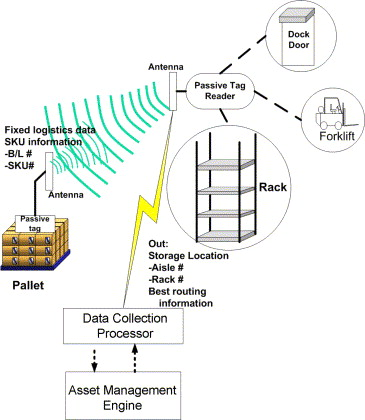
\includegraphics[width=0.5\textwidth]{../images/passive.jpg}	
		\caption{Modul proměnných logistických dat\cite{chow2006design}}
		\label{fig:passive}
\end{figure}
\ \\
K \texttt{modulu proměnných logistických dat} se vztahují ultra-širokopásmové technologie \texttt{(UWB)}, které definují přenos proměnných logistických dat mezi čtečkou a tagem, jak je znázorněno na obrázku \ref{fig:uwb}. Tento modul obsahuje kolekci aktivních tagů, čtyři čtečky \texttt{UWB} a \texttt{Hub procesor} pro sledování polohy zdrojů. \texttt{UWB} aktivní tagy se skládají z interní baterie a krátkého impulsového vysílače umožňujícího vysílat na mnohem delší vzdálenost. Tag vydá krátkodobý pulzní signál několikrát za sekundu. \texttt{UWB} čtečky přijímají signály a posílají je do Hub procesoru. S logickým nastavením triangulace rozdílného čtení \texttt{UWB} čteček lze vypočítat přesné (x, y, z) souřadnice aktivního tagu. Přitom je koordinace zdrojů ve skladu přesně vypočítaná. Takové koordinace zdrojů budou předány \texttt{sledovacímu modulu zdroje} pro následné zpracování \cite{chow2006design}.


\begin{figure}[H]
		\centering
		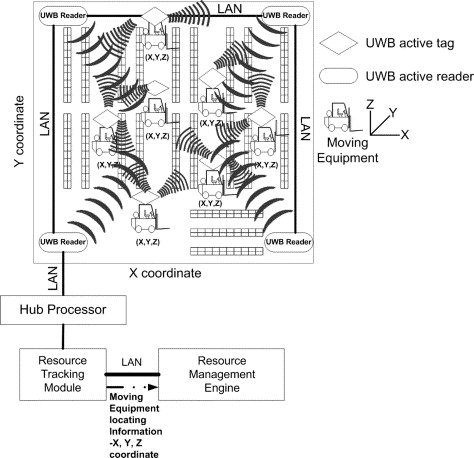
\includegraphics[width=0.6\textwidth]{../images/uwb.jpg}	
		\caption{Modul proměnných logistických dat\cite{chow2006design}}
		\label{fig:uwb}
\end{figure}


\subsection{Sledování}
\texttt{Modul sledování zdrojů} je server, který uloží všechny údaje aktivních tagů a poskytuje výkonné prostředí pro manipulaci s daty, filtruje a předává veškeré užitečné údaje řízení zdrojů pro formulování obchodní logiky a rozhodování. To je základem pro řízení zdrojů pro provádění činností včetně řízení zdrojů, plánování zdrojů, využívání a měření výkonnosti. Kromě výše uvedených funkcí, modul sledování je schopný převést data \texttt{UWB} na (x, y, z) souřadnice, které pak poskytují v reálném čase vizuální zobrazení přesného umístění zdroje na mapě skladu \cite{chow2006design}.

\subsection{Řízení}
\texttt{Modul řízení zdrojů} zpracovává data z aktivních tagů v reálném čase. Na základě těchto informací hledá optimální trasu a délku cesty k vyzvednutí zdrojů každým potenciálním manipulačním zařízením. V důsledku toho je vybráno zařízení nejvhodnější pro provedení úkolu \cite{chow2006design}.
	
\chapter{Popis zařízení}
	\section{Raspberry Pi}
		\texttt{Raspberry Pi} je řada malých jednodeskových počítačů, vyvíjená ve Velké Británii. Pro tento projekt se použije \texttt{Raspberry Pi 2 Model B} (viz obrázek \ref{fig:rpi2}), číslovka v názvu určuje generaci a \texttt{model B} je osazen ethernetovým portem na rozdíl od \texttt{modelu A}. \texttt{RPi} má procesor \texttt{Broadcom BCM2836 ARM Cortex-A7 Quad Core} \texttt{700 MHz} s možností přetaktovat na \texttt{900 MHz}, \texttt{1GB RAM}, 4x \texttt{USB 2.0}, \texttt{HDMI}, \texttt{4-pólový jack} a již zmiňovaný \texttt{10/100 Ethernet}. Přenosová rychlost \texttt{ethernetu} je velmi omezená, protože je napojený na \texttt{USB} řadič. V slotu \texttt{MicroSDHC} musí být \texttt{microSD} karta, protože z ní bootuje operační systém. Na desce jsou ještě umístěny 2 řady \texttt{pinů}, takzvané \texttt{GPIO} (viz obrázek \ref{fig:gpio}). \texttt{RPi} neobsahuje \texttt{RTC}, získávání aktuálního času se řeší pomocí protokolu \texttt{NTP}.
	
		\begin{figure}[H]
		\centering
		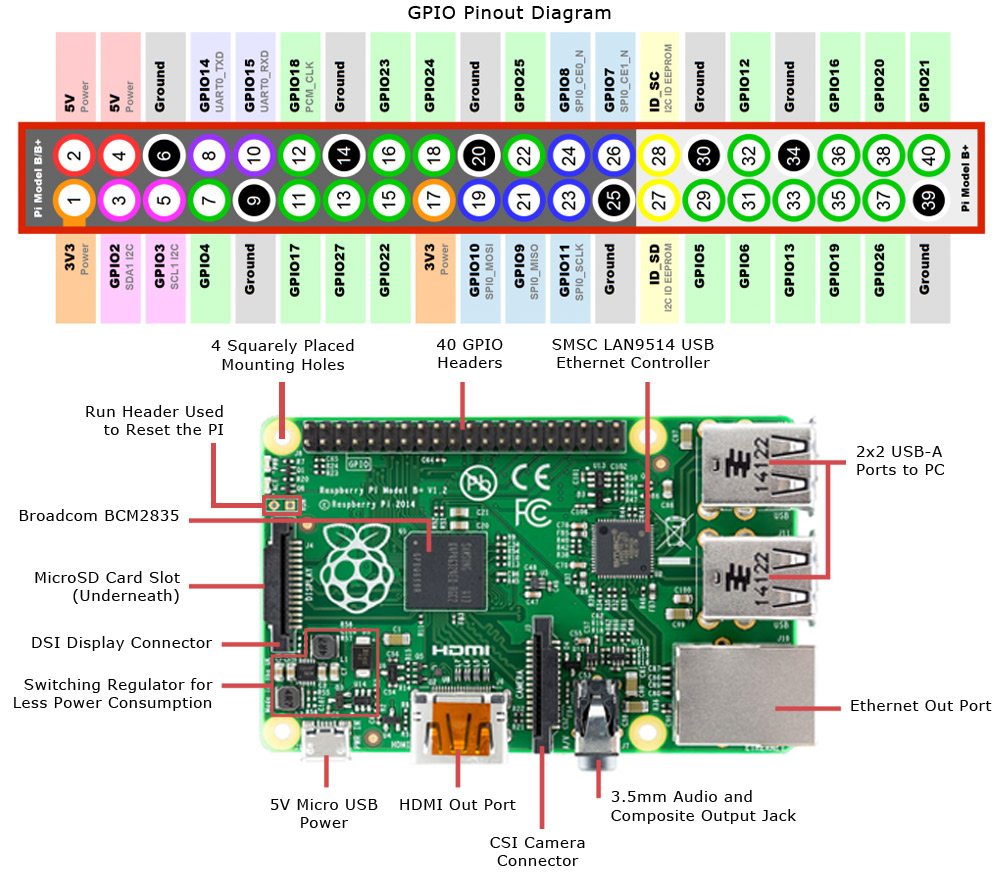
\includegraphics[width=0.85\textwidth]{../images/rpi2.jpg}	
		\caption{\texttt{Raspberry Pi 2 Model B}}
		\label{fig:rpi2}
	\end{figure}
		
	

		\subsection{GPIO}
			\texttt{GPIO (General Purpose Input/Output)} je \texttt{40 pinů} umístěných na desce ve dvouch řadách. Číslování pinů je dvojího typu \texttt{BCM} a \texttt{BOARD}, u \texttt{BCM} se počítají jen nastavitelné piny, kdežto u \texttt{BOARD} se počítají všechny.
Mezi nenastavitelné piny patří napájení \texttt{5V} (\textcolor{red}{\textbf{červená}}), napájení \texttt{3V3} (\textcolor{orange}{\textbf{oranžová}}) a \texttt{zem} (\textbf{černá}) (viz obrázek \ref{fig:gpio}).	
		
		\begin{figure}[H]
   		 	\centering
			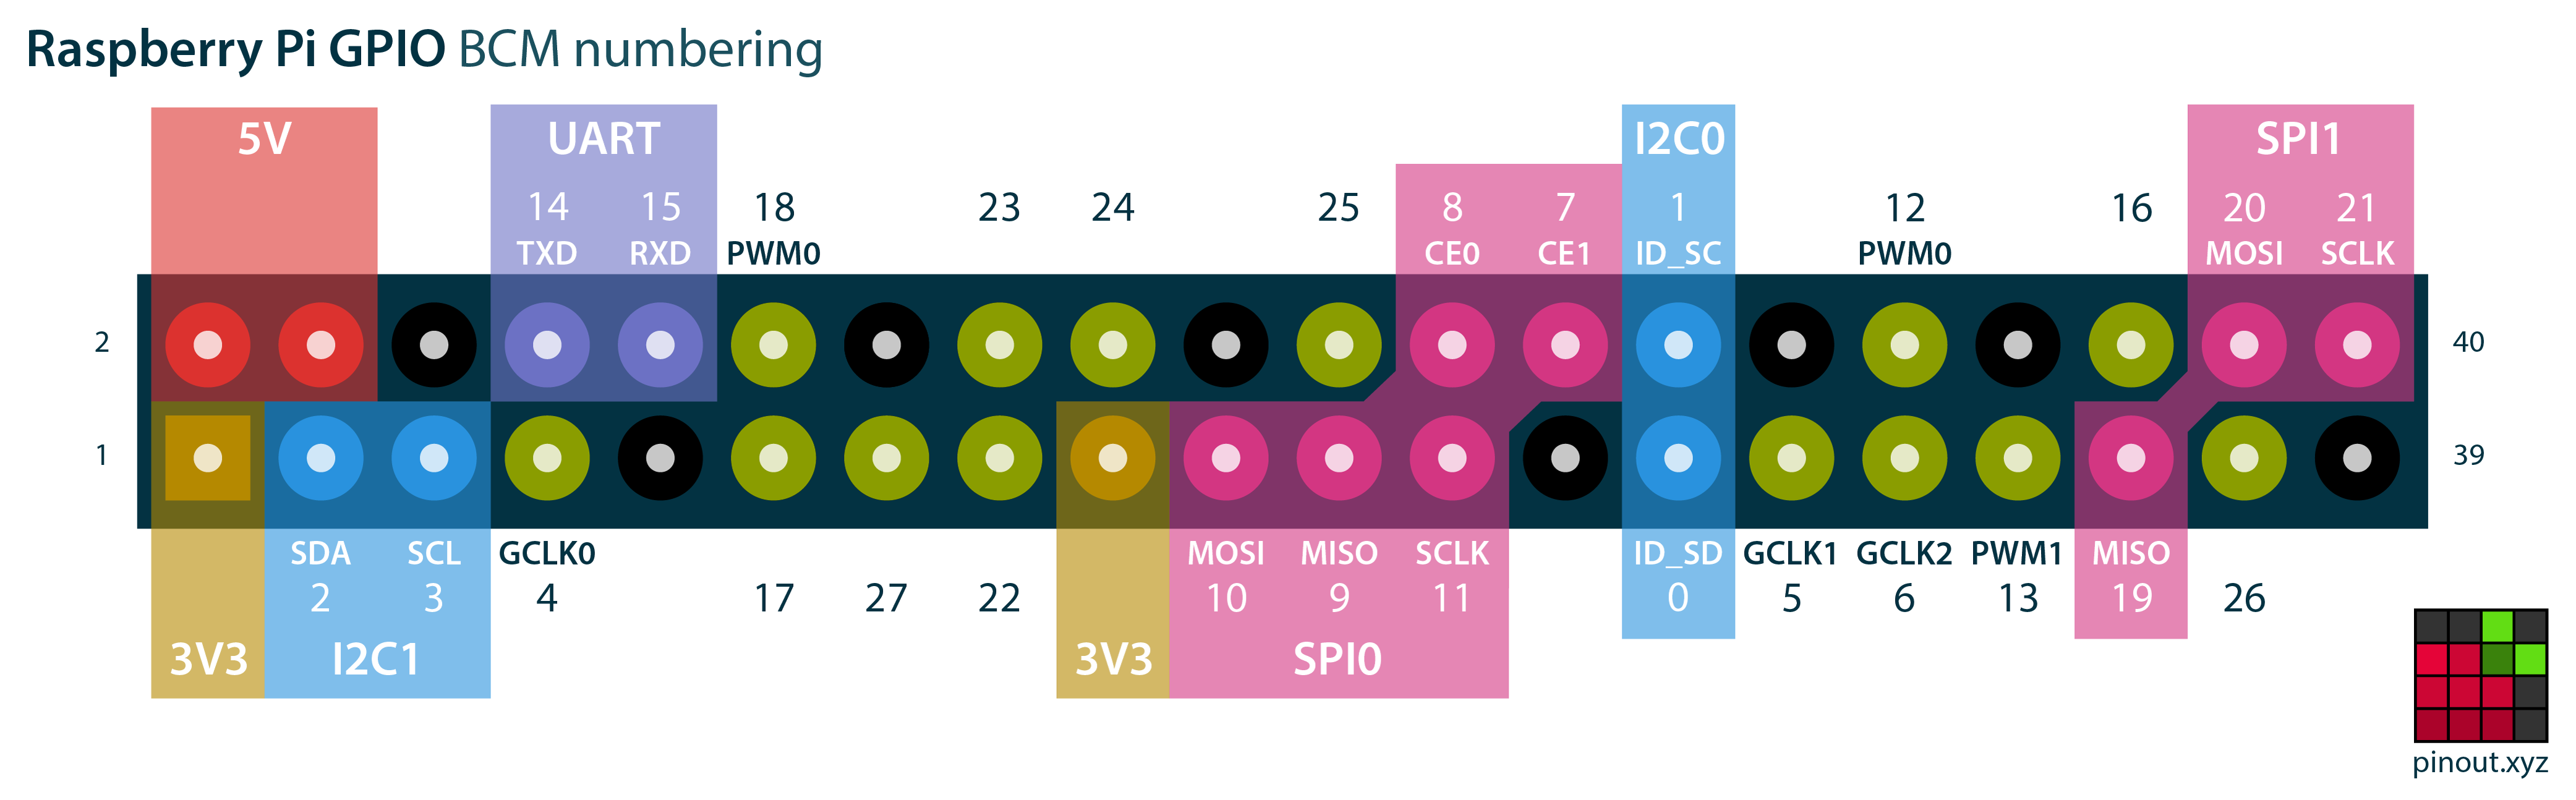
\includegraphics[width=1\textwidth]{../images/gpio.png}	
			\caption{Schéma \texttt{GPIO}}
    		\label{fig:gpio}
		\end{figure}		
		
		
		\subsection{Operační systémy}
			\subsubsection{Raspbian}
				\texttt{Raspbian} je operační systém založený na linuxové distribuci \texttt{Debian} a optimalizován pro hardware \texttt{Raspberry Pi}. Systém je vydáván ve dvou verzích Pixel a Lite, verze \texttt{Pixel} obsahuje navíc \texttt{GUI} a balíčky pro vývoj, což se promítlo na celkové velikosti \texttt{4 GB} oproti \texttt{Lite} verzi s \texttt{1,5 GB}. Pro většinu hlavních programujících jazyků je k dispozici knihovna pro ovládání \texttt{GPIO}.
			
			\subsubsection{Windows 10 IoT Core}
Verze \texttt{Windows 10 IoT Core} je určena pro minipočítače typu \texttt{Raspberry Pi}. Systém je v raném vývoji a je na stránkách \texttt{Microsoftu} k dispozici zdarma. Systém nemá uživatelské rozhraní. Spravuje se přes webové rozhraní, \texttt{Powershell} nebo na něm běží aplikace, která uživatelské rozhraní může mít. Spustit lze pouze \texttt{Universal Windows Platform (UWP)} aplikace, které je možné psát v \texttt{c\#}, \texttt{c/c++}, \texttt{Pythonu}, \texttt{Node.js} a \texttt{javascriptu}. Pro vývoj a nahrání \texttt{UWP} aplikace je zapotřebí mít \texttt{Visual Studio 2015}.
			
\section{RFID}
\texttt{RFID} představuje technologii identifikace pomocí radiofrekvenčních vln. Jedná se v podstatě o generaci identifikátorů navržených (nejen) k identifikaci zboží, navazujících na systém \texttt{čárových kódů}. Identifikace a dohledatelnost je možná celosvětově, a to při dodržení standardu dat \texttt{EPC Global} a s využitím internetového rozhraní \texttt{EPC Global Network}. \texttt{EPC} o délce \texttt{96 bitů} nabízí dostatečný číselný prostor 268 milionům výrobců produkujícím každý 16 milionů druhů výrobků (tříd), přičemž v každé třídě je prostor pro 68 miliard sériových čísel \cite{dolevcek2010identifikace}.

\subsection{Základní princip}
Technologie \texttt{RFID} pracuje na principu radaru. Transpondéry (tagy) mohou být jak aktivní, tak pasivní. Čtečka nejprve vysílá na svém nosném kmitočtu elektromagnetickou vlnu, která je přijata anténou pasivního transpondéru. Indukované napětí vyvolá elektrický proud, který je usměrněn a nabíjí kondenzátor v transpondéru. Uložená energie je použita pro napájení logických a rádiových obvodů transpondéru. Když napětí na kondenzátoru dosáhne minimální potřebné úrovně, spustí se logický automat či mikroprocesor a transpondér začne odesílat odpověď čtečce. Vysílání \texttt{transpondéru} je realizováno zpravidla pomocí dvoustavové \texttt{ASK} modulace, která je realizována změnou zakončovací impedance antény transpondéru. Odrazy, které vznikají změnou \texttt{impedance} antény, jsou detekovány čtečkou do binární podoby. Řízení komunikace a jednotlivých stavů komunikačního řetězce je definováno příslušnou \texttt{ISO} normou \cite{dolevcek2010identifikace}.


\subsection{Forma tagu}
\texttt{RFID} tag - paměťový \texttt{radiofrekvenční} čip nesoucí datovou informaci, který komunikuje bezkontaktně a bez přímé viditelnosti se snímačem - nejčastěji v podobě etikety nebo štítku. Provedení (tvar, rozměry, materiál) se mohou velmi lišit dle požadavků aplikace. \texttt{RFID} tag se skládá z vlastního čipu, antény, propojení a zapouzdření, případně baterie. Čip definuje kapacitu a typ \texttt{RFID} tagu, anténa stanovuje kvalitu příjmu a odesílání \texttt{radiofrekvenčního} signálu, zapouzdření ovlivňuje možnost použití v různých prostředích a životnost tagu \cite{dolevcek2010identifikace}.

\newpage
\begin{description}
\item [RFID Smart label]
- čip je umístěn na potisknutelné etiketě s možností dalších informací (text, \texttt{čárový kód}) viz obrázek \ref{fig:rfidsmartlabel}
\item [RFID wristband] - náramek na ruku obsahující \texttt{RFID} čip,  využití ve zdravotnictví k identifikaci osob.
\item [RFID karta] - čip může být zapouzdřen do plastové karty nebo předmětu typu klíčenky – např. k využití v platebních a docházkových systémech.
\item [RFID inlay] - zabudování čipu přímo do produktu, v případě kovového výrobku možnost oddělující vrstvy kvůli rušení.
\end{description}

\begin{figure}[H]
   		 	\centering
			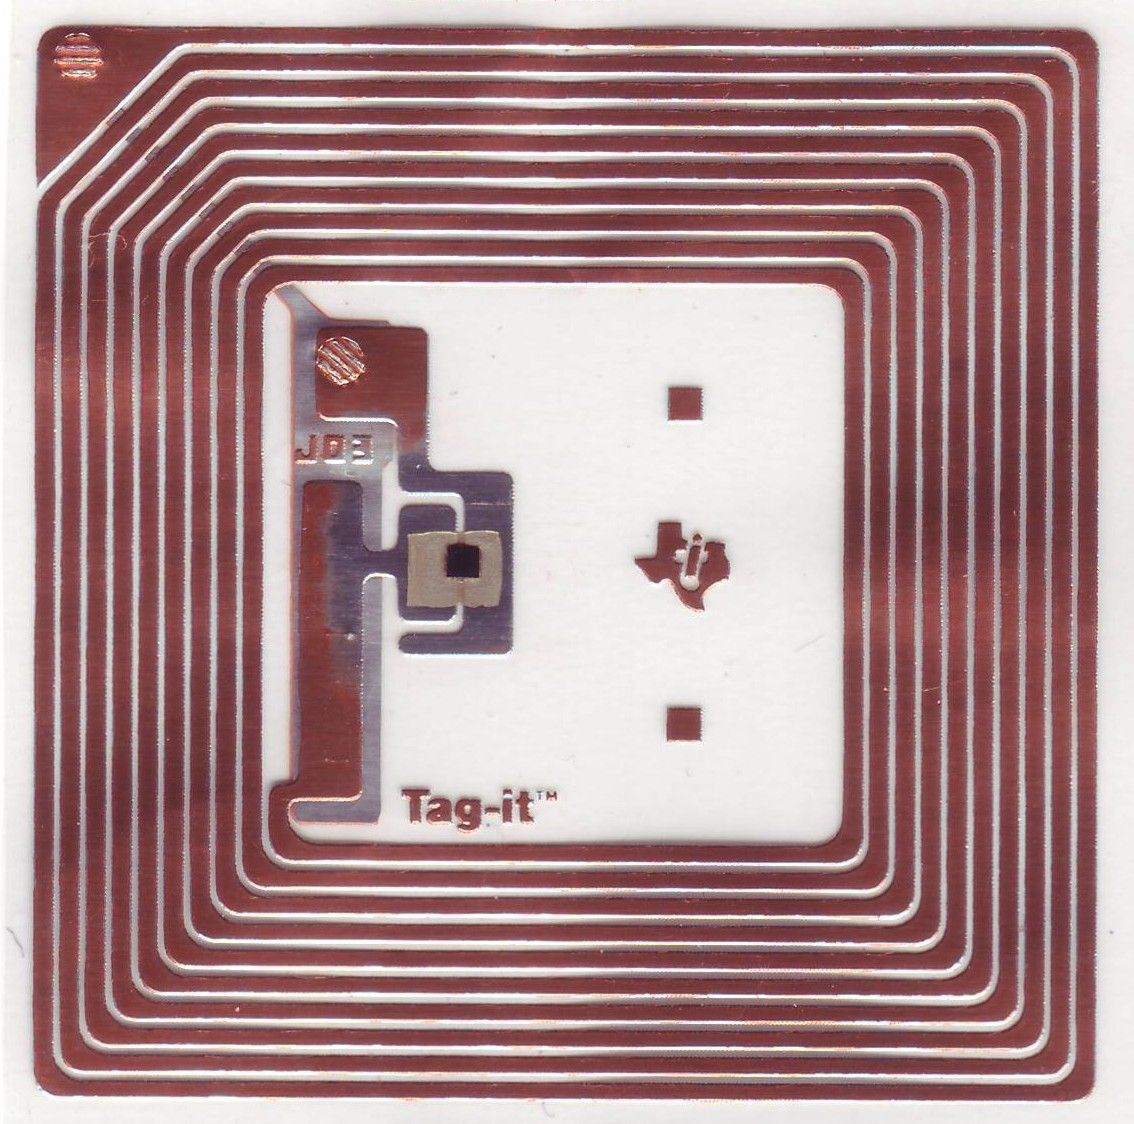
\includegraphics[width=0.6\textwidth]{../images/rfid_smart_label.jpg}	
			\caption{Pasivní HF RFID}
    		\label{fig:rfidsmartlabel}
		\end{figure}


\subsection{Frekvenční pásma}
Systémy \texttt{RFID} pracují s různými frekvencemi, přičemž frekvence ovlivňuje rychlost čtení a zápisu, dosah signálu a prostor pokrytí atd.
Více informací v tabulce \ref{table:rfid_frekvence}

\begin{table}[H]
\centering
\begin{tabular}{ c | c | p{5cm}}
 	\textbf{Frekvence} & \textbf{Dosah} & \textbf{Popis} \\ \hline\hline
    Nízká frekvence (\texttt{LF}) & \multirow{2}{*}{0,5 m} & \multirow{4}{5cm}{krátký dosah, velká anténa, pouze pro čtení, nízká přenosová rychlost, kovy a kapaliny nevadí} \\
    \texttt{125–134 kHz} &  & \\ 
    &  & \\ &  & \\ \hline
    
    Vysoká frekvence (\texttt{HF}) & \multirow{2}{*}{1 m} & \multirow{4}{5cm}{krátký dosah, velká anténa, pouze pro čtení, kapaliny znesnadňují čtení}  \\ 
	\texttt{13,56 MHz} &  & \\ 
	&  & \\ &  & \\ \hline       
	
    Velmi vysoká frekvence (\texttt{UHF}) & \multirow{2}{*}{3 m} &  \multirow{4}{5cm}{možnost číst i zapisovat, vysoká přenosová rychlost, nelze číst přes kapaliny }\\  
    \texttt{860-930 MHz} &  & \\ 
    &  & \\ &  & \\ \hline
    
    Mikrovlnná frekvence (\texttt{MW}) &  \multirow{2}{*}{10 m} & \multirow{4}{5cm}{možnost číst i zapisovat, vysoká přenosová rychlost, kapaliny a kovy příliš nevadí } \\
	\texttt{2,54 a 5,8 GHz} &  & \\ 
	&  & \\ &  & \\ \hline
\end{tabular}
\caption{Frekvenční pásma RFID}
\label{table:rfid_frekvence}
\end{table}

\newpage

\subsection{Zdroje napájení}
Čipy (tagy) se dělí na aktivní a pasivní podle toho, zda je možné informace z nich nejen číst (pasivní), ale i do nich zapisovat (aktivní). Aktivní jednotky pak musí disponovat vlastním zdrojem energie, ten obstarává miniaturní baterie \cite{dolevcek2010identifikace}.


\subsubsection{Pasivní}
Pasivní zdroje jsou nejrozšířenější, nemají vlastní baterii, napájeny jsou polem snímače. Ten periodicky vysílá pulsy prostřednictvím antény do prostoru, čip využije přijímaný signál k nabití svého napájecího \texttt{kondenzátoru} a vyšle odpověď. Pasivní tagy mají různou vzdálenost čtení od \texttt{0,5 m} do \texttt{10 m}, dlouhou životnost čipu a používají metodu \texttt{RTF (reader talk first)}. V současné době jsou nejvíce rozšířeny pasivní čipy a to zejména kvůli své nenáročnosti na obsluhu a odolnosti, velikost paměti \texttt{64-256 bitů} \cite{dolevcek2010identifikace}.


\subsubsection{Aktivní}
Aktivní zdroje mají vlastní baterii, jsou schopny vyslat svoji identifikaci. Používají se méně často než pasivní systém \texttt{RFID}. Jsou složitější, obsahují navíc i zdroj napájení a jsou schopny samostatně vysílat své identifikace - používají se proto pro aktivní lokalizaci.
Aktivní čipy vysílají samy své údaje do okolí \texttt{TTF (tag talks first)}, to umožňuje vlastní miniaturní baterie umístěná v čipu, která vydrží cca 1-5 let. Tyto čipy však kvůli baterii mají menší odolnost na teplotu a je nutné provádět výměnu baterie. Aktivní čipy mají vzdálenost čtení až \texttt{100 m}, velikost paměti na čipu může dosahovat až \texttt{100 kb} \cite{dolevcek2010identifikace}.


\subsection{Čtečka}
Snímače neboli čtečky \texttt{RFID} jsou zařízení, která dokáží zachytit vysílání aktivního nebo pasivního tagu. Čtečka nemusí pouze informace zachycovat, ale také může do tagu zapisovat. Čtečka používá pro vysílání a přijímání signálu anténu, která může být integrovaná nebo externí. Základním požadavkem na čtečku je schopnost zpracovat obrovské množství dat. Čtečky musí poznat již jednou přečtené tagy a odstranit odrazy signálů tagů od pevných překážek a musí zvládnout současně načíst velký počet tagů. S tím souvisí schopnost paralelně načítat tagy v relativně krátkém časovém intervalu \cite{dolevcek2010identifikace}.	
	
	
	
	
	
	
	
	
	
	
	
	
	
	
	
	
	
	
	
	
	
	
	
	
	
	
	
	
	
	
	
	
	
	
	
	
\chapter{Návrh řešení}

Skladový sytém se skládá ze tří propojených částí. 
První z nich je server zajišťující komunikaci mezi ostatními částmi a databází.  
Další částí je čtečka \texttt{RFID}, jejímž úkolem je umožnit skladníkům přidat a odebrat položky ze skladu.  
Poslední částí je klient umožňující uživatelům správu skladu.

		\section{Server} 
			Ze dvou možností jsem zvolil architekturu \texttt{client-server}. Hlavní výhodu vidím v tom, že na rozdíl od \texttt{peer-to-peer}, je veškerá logika soustředěná na jednom místě. Také při výskytu chyby stačí aktualizovat jen server, než aktualizovat velké množství zařízení.
			Dalším přínosem je možnost server přesunout na \texttt{cloud}. 
			Kompletní návrh komunikace viz obrázek \ref{fig:network}.
			\\\\
			Server bude postavený na \texttt{Node.js}\cite{tilkov2010node}, což je \texttt{JavaScript} v serverovém prostředí. Základem \texttt{Node.js} je javascriptový interpret \texttt{Chrome V8}, který je napsán v \texttt{C} a \texttt{C ++} se zaměřením na výkon a nízkou spotřebu paměti. \texttt{Node.js} typicky běží v jediném vlákně, to se netýká \texttt{I/O} operací, ty jsou na asynchronní. Nativní podpora formátu \texttt{JSON} se hodí pro tvorbu \texttt{REST API} nebo komunikaci s \texttt{NoSQL} databází. Komunita kolem \texttt{Node.js} vytváří spoustu užitečných modulů, které jsou k dispozici na \url{npmjs.org} \cite{tilkov2010node}.
				
				
				
		
		\begin{figure}[H]
   		 	\centering
			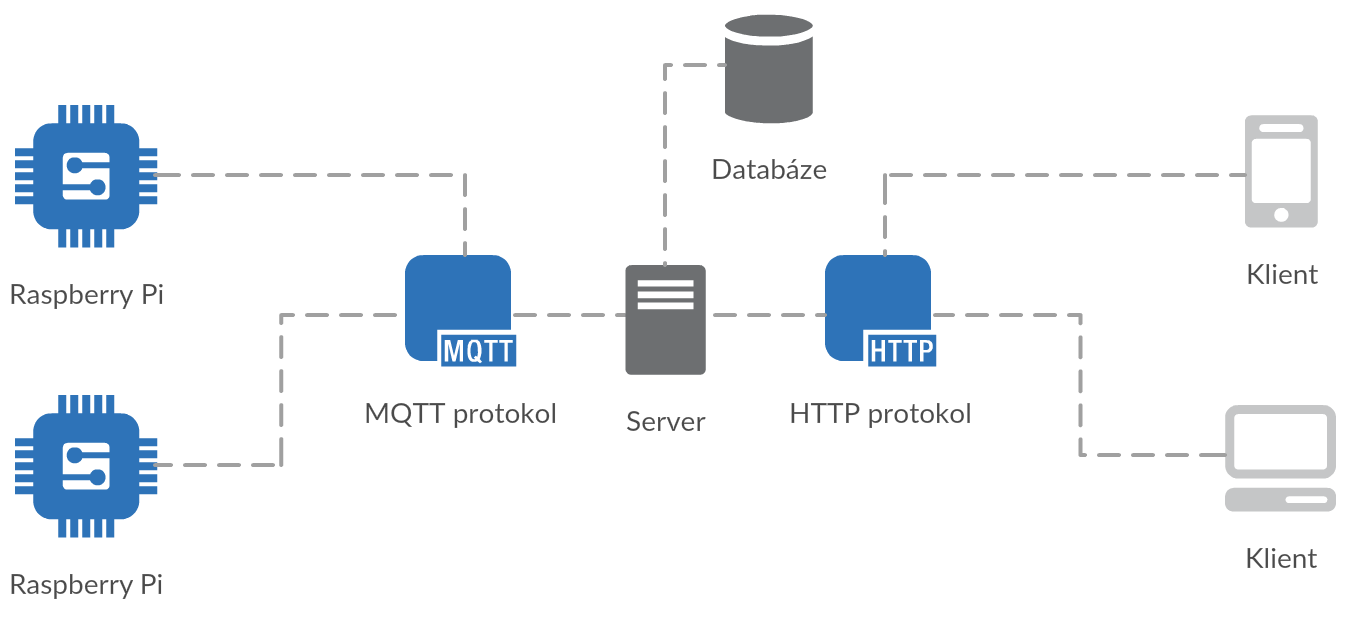
\includegraphics[width=1\textwidth]{../diagrams/network.png}	
			\caption{Návrh komunikace}
    		\label{fig:network}
		\end{figure}
		
		\subsection{Komunikace s čtečkou RFID}
			Komunikačním standardem pro \texttt{IoT} je \texttt{MQTT} protokol s velkou podporou výrobců různých zařízení, která by mohla být přínosem pro skladový systém. Takto bude skladový systém připraven na případné rozšíření.
			Z těchto důvodů jsem vybral pro komunikaci se čtečkou \texttt{RFID} protokol \texttt{MQTT}.
	
			 
			
			\texttt{MQTT} je jednoduchý a nenáročný protokol pro předávání zpráv mezi klienty prostřednictvím centrálního bodu – \texttt{brokeru}. U protokolu \texttt{MQTT} probíhá přenos pomocí \texttt{TCP} a používá návrhový vzor publisher – subscriber. Tedy existuje jeden centrální bod (\texttt{MQTT broker}), který se stará o výměnu zpráv. Zprávy jsou tříděny do tzv. témat (topic) a zařízení buď publikuje v daném tématu (publish), to znamená, že posílá data brokeru, který je ukládá a distribuuje dalším zařízením, nebo je přihlášeno k odběru tématu či témat (subscribe), a broker pak všechny zprávy s daným tématem posílá do zařízení. Jedno zařízení samozřejmě může najednou být v některých tématech publisher, v jiných subscriber \cite{maly2016mqtt}.

Samotný obsah zpráv není nijak daný ani vyžadovaný, \texttt{MQTT} je \texttt{payload agnostic}. Obsahem zprávy jsou nějaká binární data, která jsou přenesena. Nejčastěji se používá \texttt{JSON}, \texttt{BSON}, textové zprávy.\cite{maly2016mqtt}.
\\\\  
\texttt{MQTT} minimalizuje množství servisních dat. Zavádí tři úrovně \texttt{QoS}:
\begin{description}
\item [\texttt{QoS 0}] - Nejnižší úroveň znamená, že zpráva je odeslána bez potvrzení a není zaručeno její doručení (\texttt{At most once})
\item [\texttt{QoS 1}] - Prostřední úroveň říká, že zpráva je doručena alespoň jednou (\texttt{At least once})
\item [\texttt{QoS 2}] - Nejvyšší úroveň znamená, že každá zpráva je doručena právě jednou (\texttt{Exactly once})
\end{description}
\ \\
Pro zajištění zabezpečení může \texttt{MQTT} broker vyžadovat ověřování pomocí uživatelského jména a hesla. Šifrování komunikace může být řešeno pomocí \texttt{SSL}. 
Standardní port pro \texttt{MQTT} je \texttt{1883}, pro komunikaci \texttt{MQTT} přes \texttt{SSL} je výchozím portem \texttt{8883} \cite{karagiannis2015survey}.
			

		\subsection{Komunikace s klientem}
			Pro klienta potřebujeme jednotný a snadný přístup ke zdrojům. Nelze vyloučit ani přístup jiných systémů, které budou potřebovat k provozu skladový sytém. Samozřejmostí je import a export dat skladového sytému. Nejlepší volbou je otevřené \texttt{REST API}, jehož široká podpora umožní vznik různým aplikacím.


		
		\texttt{REST} není skutečným protokolem, ale architekturou pro \texttt{API}.\texttt{REST} v protokolu \texttt{HTTP} používá metody \texttt{GET}, \texttt{POST}, \texttt{PUT} a \texttt{DELETE} poskytující systém pro zasílání zpráv orientovaný na zdroje, kde lze všechny akce provádět jednoduše pomocí asynchronních příkazů \texttt{HTTP} požadavek/odpověď. Používá vestavenou hlavičku protokolu \texttt{HTTP}, která označuje formát dat v obsahu. Typ obsahu může být \texttt{XML} nebo \texttt{JSON} a závisí na serveru \texttt{HTTP} a jeho konfiguraci. Navíc může být snadno implementována v mobilních aplikacích, protože vyžaduje pouze knihovnu \texttt{HTTP}. Funkce \texttt{HTTP} mohou být plně využity v architektuře \texttt{REST} včetně cachování, autentizace a požadování typu obsahu \cite{karagiannis2015survey}.
		 
		 \texttt{RESTful} služby využívají bezpečný a spolehlivý protokol \texttt{HTTP}, který může využívat protokol \texttt{TLS/SSL} pro zabezpečení. Dnes však většina komerčních \texttt{M2M} platforem nepodporuje požadavky \texttt{HTTPS}. Namísto toho poskytují jedinečné ověřovací klíče, které musí být v záhlaví každé žádosti, aby bylo dosaženo jisté úrovně zabezpečení \cite{karagiannis2015survey}.
		 
		 



		\section{Čtečka RFID}
			Pro \texttt{Raspberry Pi} jsem zvolil operační systém \texttt{Raspbian Jessie Lite}, protože je přímo vyvíjen výrobcem. Tím je zajištěna nejlepší kompatibilita a stabilita. 
			Systém má širokou komunitu, při vyskytnutí problému bude s velkou pravděpodobností již existovat řešení.\\
			Aplikace je vyvíjena v programovacím jazyku \texttt{Python}, protože je součástí systému spolu s balíčkem \texttt{RPi.GPIO} pro řízení \texttt{GPIO}.

			\texttt{Python} je interpretovaný, interaktivní, objektově orientovaný programovací jazyk. Má pozoruhodně jednoduchou a elegantní syntaxi a přesto je univerzálním programovacím jazykem. Stejně jako mnoho jiných skriptovacích jazyků jej lze provozovat prakticky na jakémkoliv moderním počítači. \texttt{Python} program je automaticky překládán do nezávislého bajtového kódu platformy, který je pak interpretován \cite{sanner1999python}.


		\subsection{Přidat a odebrat položku}
			Přidávání a odebírání položek skladu lze vyřešit dvěma způsoby:	
			
				\begin{itemize}								
							
				\item [-] Prvním řešením je využít dvě čtečky \texttt{RFID-RC522}. Jedna čtečka by sloužila pro přidávání a druhá pro odebírání položek skladu.
				Společně s \texttt{UID} tagu by se posílal i typ akce na server. Nevýhodou tohoto řešení je zvýšení ceny celkového zařízení a zbytečná logika na zařízení.
				Pozitivum lze vidět v paralelním přidávání a odebírání položek.
				
							
				\item [-] Druhým řešením je mít jen jednu čtečku \texttt{RFID-RC522} a přepínat mezi režimy přidat a odebrat. 
				To otevírá několik otázek: Kde ukládat aktuální režim? Jak přepínat režim? Jak dát najevo aktuální režim?				
				
		
				\begin{description}				
				
				\item [Úložiště režimu] - První, co se nabízí, je ukládat režim na zařízení a serveru posílat \texttt{UID} tagu s aktuálním režimem.
				Mínusem je zbytečně přidaná logika na zařízení, které se v případě nutnosti bude obtížně aktualizovat.
				Dalším úložištěm režimu se logicky jeví server, což by přineslo možnost vzdáleně režim měnit. 
				Nevýhodou by se stala nutnost posílat aktuální režim zařízení.
				
				\item [Přepnutí režimu] - Přepínání by bylo možné pomocí tlačítka na zařízení, ale nevýhodou tohoto řešení je hygiena a výdrž mechanických částí. 			 
				Druhou možností je vyhradit si tag, který by sloužil k přepínání režimu. V neprospěch tohoto řešení je nutnost mít pro každého skladníka tag pro přepínání. 
				Poslední způsob je přepínat vzdáleně pomocí klienta, což přináší více negativ než pozitiv, hlavně z těchto důvodů: nutnost mít klienta pro každého skladníka, časová náročnost na přepnutí a možné konflikty spojené se vzájemným přepínáním režimu.
				
				\item [Zobrazení režimu] - Aktuální režim jde zobrazit třemi způsoby: \texttt{LED diodou}, bzučákem, nebo \texttt{LCD} displejem s rozlišením 16x2 znaků. Jejich samostatné použití je velmi nedostatečné a pro skladníka nepřívětivé. 


				Ideální by byla kombinace všech těchto komponentů. Zde je příklad jejich využití: Skladník má tag, který přiloží ke čtečce, ozve se pípnutí (bzučák), což ho upozorní, že tag byl načten. Dioda upozorní zablikáním na příchod odpovědi ze serveru, která se zobrazí na displeji. Na displeji se na prvním řádku objeví druh režimu a na druhém informace o odpovědi serveru.
				
				\end{description}				
				
				\end{itemize}
				\ \\
				Došel jsem k závěru, že pro přidání a odebrání skladových položek bude využita jen jedna čtečka \texttt{RFID-RC522} s přepínáním mezi režimy.
				Jelikož nemám k dispozici displej ani bzučák, bude zobrazení režimu obstarávat jen \texttt{RGB LED dioda}. Čtečka načte \texttt{UID} tagu a odešle ho na server. Tam se zjistí typ tagu a podle toho se rozhodne, jaká bude akce. Podle typu akce se objeví barevná signalizace. 
				\ \\
				Akce podle typu tagu:
				\begin{description}
					\item [položka] - Tag reprezentuje položku ve skladu. K vybrané položce se podle aktuálního režimu přičte nebo odečte kus. Při úspěšné akci se pošle příkaz k zablikání zelenou barvou.
									
					\item [režim] - Tag změní režim z přidávat na odebírat a naopak. Reakce bude podle změny: pro přidávání příkaz konstantní svícení zelenou a odebírání červenou.
					\item [neznámý] - Tento typ tagu nemá žádnou funkci. Odpověď serveru bude příkaz pro modré zablikání.
				\end{description}
				\ \\
				Při jakékoliv chybě se odešle příkaz pro zablikání červenou barvou.

				
	\section{Klient}
		Pro klienta správy skladu je důležité mít kompletní přehled. Týká se to hlavně obsluhy daného skladu, která zajišťuje příjem, výdej a přesun zboží.
		K usnadnění činnosti skladníka bude sloužit tato aplikace. V aplikaci samozřejmě nesmí chybět přidávání a upravování položek skladu.
		Mazaní položky bude možné jen v případě, pokud její počet kusů bude roven nule. Je to opatření proti schodku na skladě a i předcházení nepřesnostem při inventarizaci.
		Tag se do systému zaeviduje pouze načtením čtečky. Manuální zadání tagu nebude možné. Úprava tagu se bude týkat jen jeho typu. V případě typu položka je nutné přiřadit i konkrétní skladovou položku.
		
		Administrátor bude mít navíc k dispozici správu uživatelů a zařízení.
		Nové uživatele bude moci přidat jen administrátor. Registrace uživatelů nebude možná, protože skladový systém je určený jen skladníkům.
		Podrobný přehled všech možných akcí pro konkrétní roli viz diagram \ref{fig:mobile_app_use_case}. 
		
\begin{figure}[H]
		\centering
		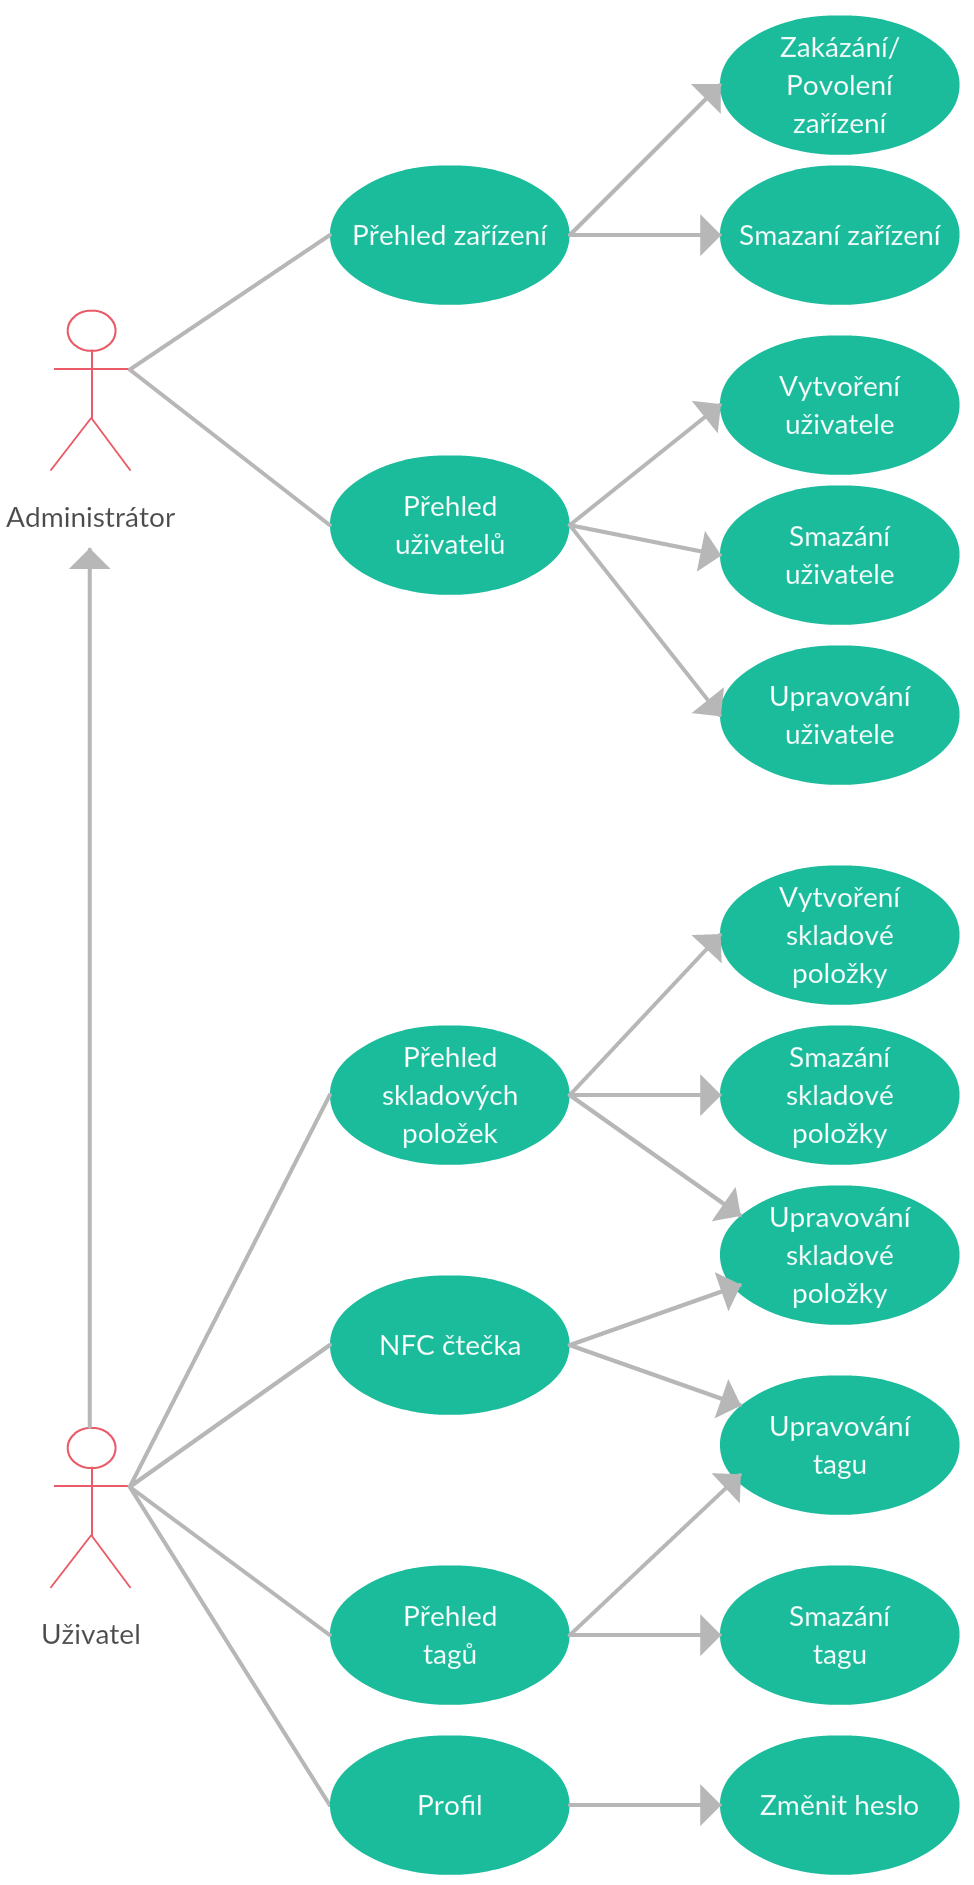
\includegraphics[width=0.8\textwidth]{../diagrams/mobile_app_use_case.png}	
		\caption{Diagram užití mobilní aplikace}
		\label{fig:mobile_app_use_case}
	\end{figure}
		
		
		
		\subsection{Platforma}
			Vybrat platformu je důležité pro uživatelskou přívětivost a použitelnost celého systému. K dispozici jsou tyto tři typy: 		
			
			\begin{description}	
				\item [Mobilní aplikace] - mobilní zařízení přináší možnost mít správu skladu neustále u sebe.
				Skoro každé zařízení dnes má \texttt{NFC}. Jelikož je \texttt{NFC} nástupcem \texttt{RFID}, existuje díky tomu zpětná kompatibilita,
			což poskytuje schopnost načíst \texttt{UID} tagu. Přiložením mobilu k tagu by skladník měl okamžitě veškeré informace o tagu případně i o položce skladu.
				
				\item [Desktopová aplikace] - se hodí pro zobrazení velkého množství dat. Bohužel správa tagů by byla velmi obtížná a komplikovaná, protože vyhledání konkretního tagu lze jen podle \texttt{UID}. 	
				\item [Webová aplikace] - obrovskou výhodou je možnost spustit aplikaci na jakémkoliv zařízení, které má webový prohlížeč. Nevýhody jsou stejné jako u desktopové aplikace.								
			\end{description}
			\ \\
			Do prostředí skladu bude pro jeho správu ideální volba mobilní aplikace. \texttt{NFC} a přenositelnost jsou důležité aspekty.
			Jelikož ve skladu probíhá spousta změn, nebudou využity možnosti notifikací, aby skladník nebyl přehlcen informacemi. Z mobilních platforem jsem zvolil \texttt{Android}, protože umožňuje vývojářům plný přístup \texttt{NFC}. 						
			Zbývající platformy jako je \texttt{Windows Phone} nebo \texttt{iOS} nejsou vhodné. 
			 \texttt{Windows Phone} je oficiálně nepoužívaná platforma, jelikož její prodej se zastavil. \texttt{iOS} je velmi omezený systém, na kterém lze \texttt{NFC} využít jen k placení a párování s \texttt{Bluetooth} sluchátky. Pro skladový systém je nevhodný. 
 
 			Vývoj bude cílen na \texttt{Androidu 6.0 Marshmallow}, protože je podle statistik nejrozšířenější verzí systému \texttt{Android}. Ke dni 5.6.2017 je na trhu zastoupen 31,2\% (viz obrázek \ref{fig:android_versions}).  
			Aplikace bude nativní, jelikož bude určená jen pro \texttt{Android}, hybridní nemá význam. Nativní vývoj probíhá v jazyku \texttt{Java}. \texttt{Java} je objektově orientovaný jazyk, jehož syntaxe je podobná \texttt{C} nebo \texttt{C++}. \texttt{Java} je interpretovaný jazyk - to znamená, že program se nepřekládá přímo do strojového kódu, ale do takzvaného bajtkódu. Bajtkód je následně interpretován na platformě Android virtuálním strojem ART, který umožňuje kompilovat část kódu aplikace už při její instalaci \cite{lacko2017vyvoj}.	
					
			
		
		\begin{figure}[H]
			\centering
			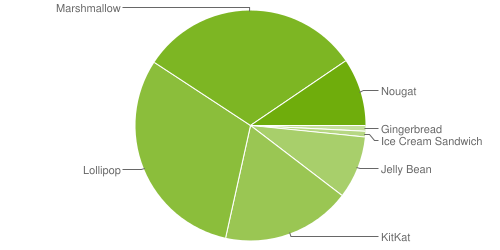
\includegraphics[width=0.7\textwidth]{../images/android_versions.png}	
			\caption{Zastoupení jednotlivých verzí systému Android ke dni 5.6.2017\\
				\centerline{\scriptsize{(zdroj: \url{https://developer.android.com/about/dashboards/index.html})}}}
			\label{fig:android_versions}
		\end{figure}		
		
		
		
				
		
		
		
	\section{Databáze}
	Pro uložení dat bude využita dokumentová databáze \texttt{MongoDB}. Dokument je v \texttt{MongoDB} základní datovou jednotkou, srovnatelnou s řádkem v relačních databázích. Jedná se o semistrukturované dokumenty vybavené indexy. Dokumenty jsou seskupovány do kolekcí, které se podobají tabulkám relačních databází, ale nemají pevně dané schéma. Protože kolekce neomezují schéma, mohou být seskupovány libovolné dokumenty v jedné kolekci. Dokumenty v kolekci by ale měly být podobné, aby bylo možné efektivní indexování. Kolekce se seskupují do databází, které jsou uloženy jako soubory v operačním systému. Jedna instance \texttt{MongoDB} může spravovat několik databází, které jsou zcela nezávislé \cite{houvzvivcka2012aplikace}.

Dokumenty jsou ukládány ve formátu \texttt{BSON}. \texttt{BSON} je binární reprezentace \texttt{JSON} formátu. \texttt{BSON} formát je bohatší než \texttt{JSON} formát a podporuje další datové typy, jako regulární výrazy, binární data nebo datum. Každý dokument má unikátní identifikátor, který je zadán uživatelem při vytváření dokumentu nebo je vytvořen \texttt{MongoDB} \cite{houvzvivcka2012aplikace}.
\\\\
Vývoj \texttt{MongoDB} je zaměřen na čtyři hlavní oblasti:
\begin{description}
\item [Flexibilita]
- \texttt{MongoDB} ukládá data jako dokumenty ve formátu \texttt{JSON}, který poskytuje datový model, jež se snadno mapuje na datové typy programovacích jazyků. Jelikož se jedná o datový model bez schématu, je jeho použití daleko snadnější než u relačních databází \cite{houvzvivcka2012aplikace}.

\item [Funkcionalita] - \texttt{MongoDB} poskytuje mnoho z funkcionalit relačních databází, jako jsou sekundární indexy, třídění, agregace apod. \cite{houvzvivcka2012aplikace}
\item [Rychlost] - Automatické dělení do fragmentů a ukládání souvisejících dat pohromadě umožňuje snadné horizontální škálování databáze a tím zvyšování výkonu bez nutnosti přerušení provozu \cite{houvzvivcka2012aplikace}.
\item [Snadné použití] -\texttt{MongoDB} je vyvíjena pro snadnou instalaci, konfiguraci, údržbu a provoz. Obsahuje jen málo konfiguračních parametrů a kdekoli je to možné, jsou nastavení prováděna automaticky \cite{houvzvivcka2012aplikace}.
\end{description}
	
	
	
	
	
	
	
	
	
	
	
	
	
	
	
	
	
	
	
	
	
	
	
\chapter{Server}
	
	Server je kombinací \texttt{MQTT} brokeru a \texttt{HTTP} serveru.
    Byl napsán v \texttt{Node.js} ve verzi \texttt{7.8}.
  Pro správu balíčku se používá \texttt{NPM}. Jeho konfiguraci naleznete v souboru \texttt{package.json}, který se nachází v kořenovém adresáři tohoto projektu. Tento soubor obsahuje všechny potřebné moduly a informace o projektu.
	

	\section{Komunikace}
		\subsection{MQTT}
			\texttt{MQTT} broker/server řeší modul \texttt{Mosca}. Je to jediný modul k dispozici pro \texttt{Node.js}. Modul \texttt{Mosca} potřebuje úložiště pro zprávy, podporovány jsou \texttt{MongoDB}, \texttt{Redis}, \texttt{Mosquitto}. Vybral jsem možnost \texttt{MongoDB}, protože je tato databáze již používaná k ukládání dat. Modul mi dává velké pole působnosti. Všechny části jako je autorizace, publikace a subscribe lze zcela přepsat, což u jiných brokerů nelze.
			
			Standardně si klient generuje náhodné \texttt{client\_id} a jelikož z uživatelského hlediska jsou takováto \texttt{ID} nepřívětivá, tak server umožní připojení jen klientům, kteří splňují tento formát.\\Každý klient, který se chce připojit k brokeru, musí jako \texttt{client\_id} splňovat tento formát \texttt{[app\_name]/[device\_id]}. \texttt{ID} klienta musí být jedinečné, aby se předešlo konfliktu při připojování k \texttt{MQTT} brokeru. 
				Název aplikace v \texttt{client\_id} umožňuje, aby se mohly připojit různé aplikace z jednoho zařízení. 

			Zařízení se po připojení automaticky zaeviduje do databáze, přitom dojde k rozdělení \texttt{client\_id} na název aplikace a \texttt{ID} zařízení, které se uloží spolu s \texttt{IP} adresou. 
			Připojené zařízení informuje server o své verzi softwaru a sériovém čísle, tyto informace pomůžou správci v rozhodnutí, které zařízení aktualizovat a nalezení konkrétního zařízení. 
			
			
		
			\subsubsection{Autorizace}
		Standardně se přístup k \texttt{MQTT} brokeru řeší přihlašujícími údaji. 
		Buď se pro všechna zařízení určí společné přihlašovací údaje, které si každé zařízení bude pamatovat, nebo každému zařízení přidělí vlastní přihlašovací údaje, což zkomplikuje správu zařízení.		
 		V případě hacknutí se u první možnosti musí měnit hesla na všech zařízeních, u druhé jen na hacknutém zařízení.
 		
 		Z tohoto důvodu jsem zvolil jiný způsob řešení.
		Zařízení se při připojení automaticky zaregistruje do databáze. Pokud již v databázi existuje, tak se zkontroluje povolení k přístupu, které přiděluje administrátor.
		V případě, že povolení nemá, je odpojen. Toto je elegantní řešení, které umožní administrátorům mít přehled o všech připojeních k \texttt{MQTT} serveru.			
		Bezpečností riziko může vzniknout ukradením \texttt{client\_id}. Tento problém lze řešit zakázáním přístupu v případě změny \texttt{IP} adresy.
		
		
		
		
	
		\subsection{REST API}
		\texttt{HTTP} server obstarává modul \texttt{Restify} framework, který slouží k tvorbě \texttt{REST API}. Díky přizpůsobení frameworku pro \texttt{API} neobsahuje šablonovací ani renderovací systém, což je znát na rychlosti zpracování požadavku.
		Také obsahuje užitečnou funkci \texttt{throttle}, při překročení 50 dotazů za sekundu dojde k zablokování zdroje žádostí.		
		
		\texttt{REST API} je umístěno na adrese \texttt{/api/v1/}, verzování standardně v \texttt{URL}. Data jsou k dispozici jen ve formátu \texttt{JSON}. 
\\\\
Popis všech dostupných \texttt{URL} adres v \texttt{API} viz tabulka \ref{table:api}.
\begin{table}[H]
\centering
\begin{tabular}{ c | c | p{6cm}}
\textbf{Metoda} & \textbf{ \texttt{URL}} & \textbf{Popis} \\ \hline\hline
 	
\texttt{GET} & \texttt{/api/v1/devices} & Vrátí všechna zařízení \\ \hline  
\texttt{GET} & \texttt{/api/v1/devices/\{id\}} & Vrací jedno zařízení \\ \hline
\texttt{PUT} & \texttt{/api/v1/devices/\{id\}} & Aktualizuje jedno zařízení \\ \hline
\texttt{DELETE} & \texttt{/api/v1/devices/\{id\}} & Odstraní jedno zařízení  \\ \hline

\texttt{GET} & \texttt{/api/v1/items} & Vrátí všechny položky \\ \hline
\texttt{POST} & \texttt{/api/v1/items} & Vytvoří novou položku \\ \hline
\texttt{GET} & \texttt{/api/v1/items/\{id\}} & Vrací jedinou položku \\ \hline
\texttt{PUT} & \texttt{/api/v1/items/\{id\}} & Aktualizuje jednu položku \\ \hline
\texttt{DELETE} & \texttt{/api/v1/items/\{id\}} & Odstraní jednu položku \\ \hline

\texttt{GET} & \texttt{/api/v1/tags} & Vrátí všechny tagy  \\ \hline
\texttt{GET} & \texttt{/api/v1/tags/\{id\}} & Vrátí jednu značku \\ \hline
\texttt{PUT} & \texttt{/api/v1/tags/\{id\}} & Aktualizuje jednu značku \\ \hline
\texttt{DELETE} & \texttt{/api/v1/tags/\{id\}} & Odstraní jednu značku \\ \hline
\texttt{GET} & \texttt{/api/v1/tags/uid/\{uid\}} & Vrátí jednu značku \\ \hline

\texttt{GET} & \texttt{/api/v1/users} & Vrátí všechny uživatele \\ \hline
\texttt{POST} & \texttt{/api/v1/users} & Vytvoří nového uživatele \\ \hline
\texttt{GET} & \texttt{/api/v1/users/\{id\}} & Vrátí jednoho uživatele \\ \hline
\texttt{PUT} & \texttt{/api/v1/users/\{id\}} & Aktualizuje jednoho uživatele \\ \hline
\texttt{DELETE} & \texttt{/api/v1/users/\{id\}} & Odstraní jednoho uživatele \\ \hline

\texttt{GET} & \texttt{/api/v1/account/} & Vrátí přihlášeného uživatele  \\ \hline
\texttt{PUT} & \texttt{/api/v1/account/password/} & Změní heslo přihlášeného uživatele \\ \hline    
\end{tabular}
\caption{\texttt{REST API v1}}
\label{table:api}
\end{table}

			\subsubsection{Stavové kódy HTTP}
			\texttt{HTTP} umožňuje použít celou škálu kódů s jasnou sémantikou. V \texttt{REST API} využijeme jen několik z nich:
\begin{description}
\item [\texttt{200 OK}] - Zpracování požadavku proběhlo bez problému.
\item [\texttt{201 Created}] - Zpracování požadavku proběhlo bez problému. Záznam byl vytvořen. 
\item [\texttt{204 No Content}] - Zpracování požadavku proběhlo bez problému. Záznam byl smazán.
\item [\texttt{400 Bad Request}] - Požadavek nebyl zpracován. Důvodem může být serverem neznámý požadavek nebo špatná vstupní data.
\item [\texttt{401 Unauthorized}] - Požadavek nebyl zpracován. Žadatel nebyl autorizován.
\item [\texttt{403 Forbidden}] - Požadavek nebyl zpracován. Žadatel nemá potřebná práva.
\item [\texttt{404 Not Found}] - Požadovaný záznam nebyl nalezen.
\item [\texttt{500 Internal Server Error}] - Požadavek nebyl zpracován. Nastala nečekaná chyba.
\end{description}

	\subsubsection{Autentizace}
		Autentizace je proces ověření pravosti přihlašovacích údajů, tento proces řeší modul \texttt{Passport}, jehož jediným účelem je ověřování požadavků, a který to dělá přes rozšiřitelnou sadu zásuvných modulů, známých jako \texttt{strategie}. 
		Existují \texttt{strategie} pro \texttt{autentizaci} pomocí \texttt{OAuth}, \texttt{Facebook}, \texttt{Twitter}, \texttt{OpenID} a spoustu dalších.		
		Vybral jsem strategii \texttt{HTTP Basic} hlavně kvůli rychlé implementaci a jisté podpoře klienta.
		Použité \texttt{HTTP Basic auth} funguje velmi jednoduše: jméno a heslo je posláno jako textový řetězec, který se skládá ze jména, dvojtečka a heslo, pak se celé zakóduje \texttt{Base64}, poté vložíme do \texttt{HTTP} hlavičky.
Příklad přidané autentizace do hlavičky \texttt{HTTP}:
\begin{verbatim}
		Authorization:Basic a29obDpoZXNsbzM=
\end{verbatim}
Aby byla zajištěna bezpečnost, počítá se s šifrovanou komunikací, jinak lze heslo lehce odposlechnout.

	\subsubsection{Autorizace}
	Autorizace je proces ověření potřebných oprávnění pro přístup uživatele k datům. Oprávnění je možné získat s přidělenou rolí.
	
	Každý uživatel musí mít alespoň jednu roli. Možné role jsou \texttt{admin} a \texttt{user}. 
	Uživatel s rolí \texttt{user} má přístup jen ke správě skladových položek a správě tagů. 
	Zato administrátor má navíc k dispozici správu zařízení a správu uživatelů s rolí \texttt{user}.
	
	Od spuštění serveru existuje účet s uživatelským jménem \uv{admin}.
	Tento účet se vyváří automaticky a nelze smazat. Dalším specifikem účtu jsou rozšířená práva pro správu uživatele s rolí \texttt{admin}.
	
	
	\subsubsection{Dokumentace}
	Dokumentace je řešena frameworkem \texttt{Swagger} nejrozšířenějším nástrojem pro vývojáře \texttt{API}, který umožňuje vývoj napříč životním cyklem \texttt{API} od návrhu či dokumentace až po testování či zavádění.	
	Modul \texttt{swagger-jsdoc} umožňuje z komentářů vygenerovat \texttt{Swagger specifikaci} ve formátu \texttt{JSON}, která se předá  \texttt{Swagger UI}. 
	Zvolil jsem generování z komentářů, abych měl popis a implementaci na jednom místě a zabránilo se nekonzistenci.
	\texttt{Swagger UI} je webová stránka, která se automaticky generuje ze \texttt{Swagger specifikace}. Umožní komukoliv si prohlédnout a vyzkoušet \texttt{API} rozhraní, aniž by byla použita logika implementace.
	\\\\
	Dokumentace je dostupná na adrese \texttt{/api/docs/}



	\section{Databáze}
	Pro jednodušší přístup k dokumentům v \texttt{MongoDB} databázi se použije modulu \texttt{Mongoose}. Nabízí podobnou funkcionalitu jako různé \texttt{ORM} frameworky.
	\texttt{Mongoose} nabízí nástroje pro \texttt{CRUD} operace (vytváření, čtení, editaci a mazání) nebo třeba umožňuje provádět validaci před vložením dokumentu do kolekce. V \texttt{Mongoose} všechno začíná u schématu. Každé schéma mapuje kolekci \texttt{MongoDB} a definuje strukturu dokumentů v rámci této kolekce. Každý klíč ve schématu definuje vlastnost v dokumentech, kterému se musí přiřadit odpovídající datový typ. Dále lze klíči nastavit max/min hodnota, max/min délka řetězce, \texttt{trim}, \texttt{index}, povinný údaj, výchozí hodnotu atd. Schéma se musí převést na model, s nímž pak lze pracovat.
	
	Všem schématům jsem nastavil striktní dodržování struktury a přidal časová razítka vytvoření a úpravy dokumentu.
	Verzování dokumentů jsem vypnul, protože jsem ho nepotřeboval a naopak jsem povolil virtuální vlastnosti, které nejsou uloženy v databázi, ale dopočítávají se.
	
	Databáze obsahuje jen nejnutnější údaje, aby se dala prezentovat funkčnost skladového systému. 	
	
	
	\subsubsection{Položka}
Položce jsem určil tyto vlastnosti: \texttt{name}, \texttt{description} a \texttt{amount}. Ostatní údaje jako cena, expirace a šarže jsou aktuálně nedůležité. Vlastnost \texttt{amount} má výchozí hodnotu 0, protože množství položky lze zadat jen při editaci položky. 
Schéma položky:	
\begin{verbatim}
{
    name: { type: String, trim: true, minlength: 3,
            maxlength: 200, required: true },
    description: { type: String, trim: true, maxlength: 2000 },
    amount: { type: Number, default: 0, min: 0, required: true }
}
\end{verbatim}

	\subsubsection{Tag}
Tagu jsem přidělil tyto vlastnosti: \texttt{uid}, \texttt{type} a \texttt{item}. Vlastnost \texttt{uid} má omezení na 8 znaků, aby se nevkládalo \texttt{uid} z jiných typů tagů, které nejsou podporovány čtečkou \texttt{RFID}.
Vlastnost \texttt{item} může obsahovat \texttt{\_id} položky, \texttt{autopopulate} je proces automatického nahrazení specifikované cesty v dokumentu s dokumentem z jiné kolekce.
Schéma tagu:
\begin{verbatim}
{
    uid: { type: String, lowercase: true, trim: true,
            minlength: 8, maxlength: 8, required: true,
            unique: true },
    type: { type: String, enum: ['unknown', 'mode', 'item'],
            default: 'unknown', required: true },
    item: { type: Schema.Types.ObjectId, ref: 'Item',
            index: true, autopopulate: true }
}
\end{verbatim}
	
	\subsubsection{Uživatel}
Uživateli jsem stanovil tyto vlastnosti: \texttt{username}, \texttt{password}, \texttt{firstname}, \texttt{lastname} a \texttt{roles}. Pro lepší práci s uživatelem jsem přidal virtuální vlastnost \texttt{fullname}, která se skládá z \texttt{firstname} a \texttt{lastname}.\\
Vlastnost \texttt{roles} musí obsahovat pole práv, může nabývat práv \texttt{admin} a \texttt{user}.
Schéma uživatele:
\begin{verbatim}
{
    username: { type: String, lowercase: true, trim: true,
            minlength: 3, maxlength: 20, required: true,
            unique: true },
    password: { type: String, default: '', required: true,
            select: false },
    firstname: { type: String, default: '', trim: true,
            maxlength: 30 },
    lastname: { type: String, default: '', trim: true,
            maxlength: 30 },
    roles: { type: [{ type: String, enum: ['admin', 'user'] }],
            required: true }
}
\end{verbatim}
	
	\subsubsection{Zařízení}

Zařízení jsem určil tyto vlastnosti: \texttt{device\_id}, \texttt{name}, \texttt{version}, \texttt{description}, \texttt{status}, \texttt{allowed}, \texttt{serial\_number}, \texttt{ip\_address} a \texttt{metadata}. 
Vlastnost metadata je typu \texttt{Mixed}, což znamená, že může obsahovat cokoliv.
Důvodem jsou četná zařízení, která potřebují uložit různá data. 
Také obsahuje virtuální vlastnost \texttt{client\_id}, která vzniká spojením \texttt{name}, lomítka a \texttt{device\_id}.\\
Vlastnost \texttt{status} může obsahovat jen hodnoty z \texttt{enum}, je to obdoba číselníků z relační databáze. 
Celé schéma zařízení:

\begin{verbatim}
{
    device_id: { type: String, trim: true, required: true },
    name: { type: String, trim: true, required: true },
    version: { type: String, trim: true},
    description: { type: String, trim: true },
    status: { type: String,
            enum: ['active', 'inactive', 'error'],
            default: 'inactive', required: true },
    allowed: { type: Boolean, default: false },
    serial_number: { type: String, trim: true },
    ip_address: { type: String, trim: true },
    metadata: { type: Schema.Types.Mixed }
}
\end{verbatim}



	
	
\section{Konfigurace}
		Konfiguraci obstarává modul \texttt{config}, který načte konfigurační soubory ze složky \texttt{./config} typicky umístěné v kořenovém adresáři aplikace. 	
		Modul podporuje velké množství konfiguračních souborů: \texttt{json}, \texttt{js}, \texttt{xml}, \texttt{toml}, \texttt{yaml} a další.
		Ze souboru \texttt{config/default.[format]} dědí všechny ostatní konfigurační soubory.
		Formát konfiguračního souboru byl vybrán \texttt{js}, pro možnost načíst data ze souboru \texttt{package.json}, který slouží jako konfigurační soubor pro správce modulů \texttt{NPM}.	
			
		V \texttt{Node.js} lze při spuštění nastavit parametr \texttt{NODE\_ENV}, který určuje v jakém prostředí běží. Výchozí hodnotou je \texttt{development}.
		Některé moduly se přizpůsobují prostředí, např. podle \texttt{NODE\_ENV} změní level logování. 
		Modul \texttt{config} vybírá konfigurační soubor podle \texttt{NODE\_ENV}, např. při \texttt{NODE\_ENV=test} se vybere soubor \texttt{config/test.js}.
\\\\
		Ukázka konfiguračního souboru \texttt{config/default.js}:	
\begin{verbatim}
{
    name: 'BPINI',
    version: package.version,
    host: '127.0.0.1',
    port: {
        http: 80,
        mqtt: 1883
    },
    logger: {
        level: 'info',
        path: './logs/bpini.log'
    },
    mongodb: {
        uri: 'mongodb://127.0.0.1:27017/warehouse',
        options: {}
    },
    api: true
}
\end{verbatim}
\ \\
	V konfiguračním souboru lze nastavit  \texttt{host} a  \texttt{porty} pro \texttt{MQTT} a \texttt{HTTP}. Další nastavení se týká umístění a level logování. Pro připojení databáze musí do parametru \texttt{uri} zadat \texttt{Connection string} podle standardního formátu \texttt{MongoDB URI}. Dodatečná nastavení jako \texttt{ssl}, \texttt{connectTimeoutMS} atd. se nastavují přes parametr \texttt{options}. 
	
	Spolu se servem se spouští i \texttt{API}, automatické spuštění můžeme zakázat změněním parametrů \texttt{api} na false. \texttt{API} lze také spustit zcela samostatně.	
	
	
	\section{Logování}
	Logování zajišťuje modul \texttt{Bunyan}. Velmi často se používá a má podporu v ostatních modulech např. \texttt{Restify}.
	Typ logu je \texttt{rotating-file}, znamená to, že každý den se vytvoří nový soubor logu, který se uchová po dobu jednoho týdne.
	\texttt{Bunyan} je charakteristický logováním ve formátu \texttt{JSON}, díky tomu je lepší práce s logy např. vyhledávání.
	Propojení s \texttt{Restify} zajišťuje logování všech požadavků a odpovědí serveru. 
	
	
	
	
	
	
	
	
	
	
	
	
	
	

	
	
\chapter{Čtečka RFID}
	\section{Sestrojení}
	
		Pro sestrojení čtečky \texttt{RFID} jsem použil tyto hlavní komponenty: \texttt{Raspberry Pi 2}, \texttt{RFID-RC522} a \texttt{RGB LED diodu}. 
		Kompletní model zapojení viz obrázek \ref{fig:reader_rfid_diagram}, schéma je k dispozici v manuálu.
		
\begin{figure}[H]
		\centering
		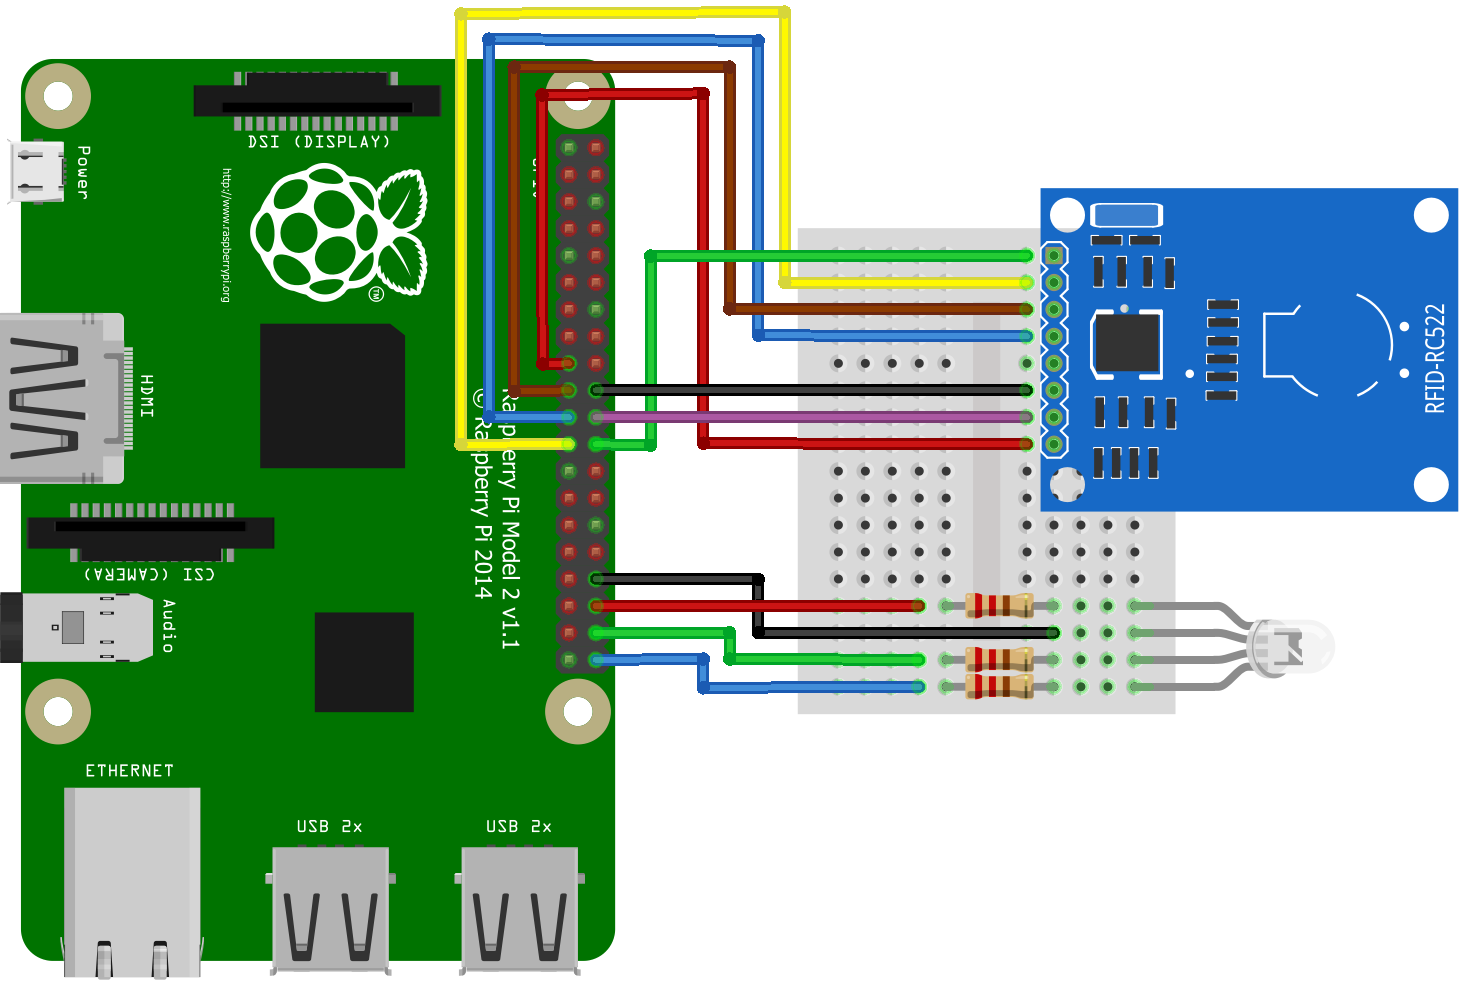
\includegraphics[width=0.9\textwidth]{../diagrams/reader_rfid_diagram_bb.png}	
		\caption{Model zapojení \texttt{RFID-RC522} a \texttt{RGB LED} do \texttt{GPIO}}
		\label{fig:reader_rfid_diagram}
	\end{figure}		
		
				
		\section{Zapojení RFID-RC522}
Čtečka \texttt{RFID-RC522} (viz obrázek \ref{fig:rfid_rc522}) se k \texttt{Raspberry Pi} zapojí přes \texttt{GPIO}. 
\begin{figure}[H]
		\centering
		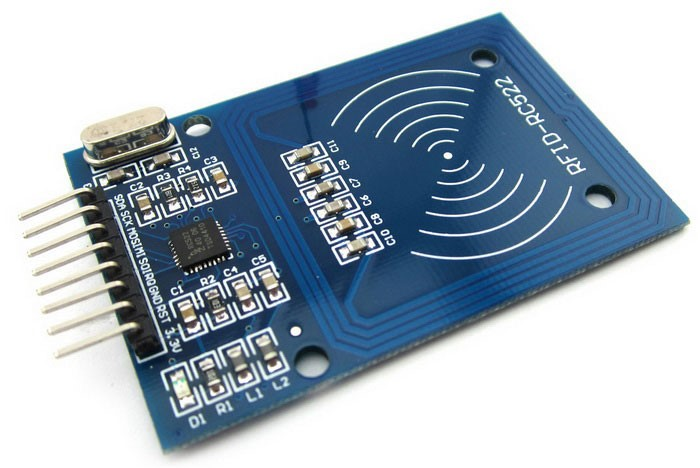
\includegraphics[width=0.7\textwidth]{../images/rfid_rc522.jpg}	
		\caption{Čtečka \texttt{RFID-RC522}}
		\label{fig:rfid_rc522}
	\end{figure}
\ \\
Komunikace probíhá přes \texttt{SPI}, což je synchronní sériový datový protokol používaný pro komunikaci mezi mikroprocesory nebo s periferními zařízeními.
Při komunikaci přes \texttt{SPI} je vždy jedno zařízení hlavní, které řídí periferní zařízení \cite{upton2014raspberry}.
Komunikaci \texttt{SPI} se vždy skládá z těchto pinů (viz obrázek \ref{fig:spi}):			
\begin{itemize}[noitemsep]
\item [-] \texttt{MISO (Master Slave Out)} - \texttt{slave} linka pro odesílání dat do \texttt{master}
\item [-] \texttt{MOSI (Master Out Slave In)} - \texttt{master} linka pro odesílání dat do periferií
\item [-] \texttt{SCK (Serial ClocK)} - hodinové pulsy, které synchronizují přenos dat 
\end{itemize}
						
	\begin{figure}[H]
		\centering
		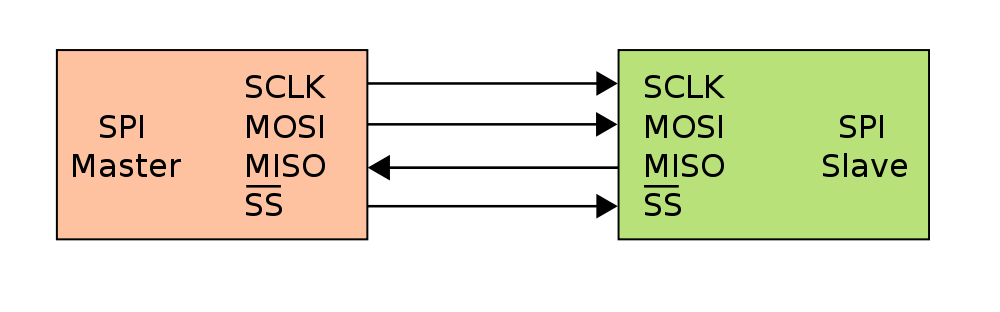
\includegraphics[width=0.7\textwidth]{../images/spi.png}	
		\caption{Zapojení sběrnice \texttt{SPI}: řídicí (\texttt{master}) a podřízené (\texttt{slave}) zařízení}
		\label{fig:spi}
	\end{figure}
\ \\
\texttt{GPIO} má vyhrazené piny pro \texttt{SPI} (viz obrázek \ref{fig:gpio}). \texttt{RFID-RC522} potřebuje navíc napájení \texttt{3V3}, \texttt{GND} a \texttt{pin 22} (podle \texttt{BOARD}) pro \texttt{RST} (Reset). Kompletní zapojení je popsáno na schématu (viz obrázek \ref{fig:reader_rfid_diagram}).






\subsection{Zapojení RGB LED diody}
	Pro rozsvícení \texttt{RGB LED diody} potřebujeme 4 piny (viz obrázek \ref{fig:rgb_led_dioda}). Nejdelší pin je \texttt{GND}, nalevo od \texttt{GND} je pin pro červenou, napravo pro zelenou a modrou barvu.
	\begin{figure}[H]
		\centering
		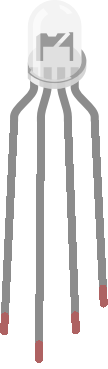
\includegraphics[width=0.09\textwidth]{../images/rgb_led_dioda.png}	
		\caption{\texttt{RGB LED dioda}}
		\label{fig:rgb_led_dioda}
\end{figure}
\ \\
Parametry \texttt{RGB LED diody} pro provoz jsou: proud až \texttt{20 mA}, napětí v propustném směru až \texttt{1,7 V}.
Před piny určující barvu je potřeba zapojit \texttt{rezistory} \cite{voda2016rezistor}, protože \texttt{GPIO} dodává napětí \texttt{3,3 V}.
\texttt{Rezistory} se používají na ochranu diody před poškozením. 
Pro výpočet potřebného odporu \texttt{rezistoru} se používá \texttt{Ohmův zákon}. Udává vztah mezi \texttt{U (napětí)}, \texttt{I (proud)} a  \texttt{R (odpor)} v obvodu. Matematicky formulovaný je takto:
\[ U = R * I \]
\ \\
Z toho vyplývá také vztah:
\[ R = U/I \]
\[ 80=(3.3-1.7)/0.02 \]
\texttt{Rezistor} s odporem \texttt{80 Ohm} je těžko dostupný, proto jsem použil nejčastěji používaný \texttt{rezistor} s \texttt{200 Ohm}.
Zapojení je vidět na schématu (viz obrázek \ref{fig:reader_rfid_diagram}).


	\section{Aplikace}
Aplikace je napsaná v jazyce \texttt{Python} ve verzi \texttt{2.7}, abych zajistil správnou funkčnost všech balíčků. Všechny potřebné balíčky pro spuštění aplikace jsou umístěny v souboru \texttt{requirements.txt}, který je umístěný v kořenovém adresáři.


	\subsection{Načtení UID tagu}
Pro načtení \texttt{UID} je zapotřebí řídit \texttt{GPIO} na \texttt{Raspberry Pi}, to zajišťuje balíček \texttt{RPi.GPIO}. Vybrán byl tento balíček, protože je to oficiální knihovna od tvůrců \texttt{Raspberry Pi} a je součástí operačního systému.
Balíček \texttt{spidev} umožňuje komunikovat se zařízením \texttt{SPI} s \texttt{Raspberry Pi} jako hlavním zařízením. 
Dalším balíčkem je \texttt{rc522}. Jeho hlavní účel je ovládat přes \texttt{SPI} součástku \texttt{RFID-RC522}. Tento balíček byl využit hlavně pro načtení \texttt{UID}, které jsem musel poupravit, jelikož docházelo k neustálému načítání tagu. 
Pro další načtení \texttt{UID} je nutné mít za sebou dva neúspěšné pokusy o načtení tagu, což znamená, že tag je odebrán z dosahu čtečky a nedochází tak k vícenásobnému načtení, než je potřeba.



	\subsection{Komunikace}
	Pro komunikaci s \texttt{MQTT} brokerem jsem použil oficiální balíček od tvůrců \texttt{MQTT}.
	Balíček \texttt{Paho} vyžaduje před připojením určit klient \texttt{ID}.
	Klient \texttt{ID} je vygenerováno z názvu aplikace a \texttt{ID} zařízení. 
	Jako \texttt{ID} se bere \texttt{MAC} adresa zařízení, tím se zajistí jedinečnost. \texttt{MAC} adresu má každé zařízení se síťovou kartou.
	\\\\
	Ukázka klient \texttt{ID} pro čtečku \texttt{RFID}:
	\begin{verbatim}
		reader_rfid/b827eb7c800d
	\end{verbatim}		
	\ \\
	Klient \texttt{ID} se používá v tématu (topicku) zpráv, aby se identifikovalo od koho a komu je zpráva určená.		
	Zde je ukázka (viz obrázek \ref{fig:mqtt_communication}) komunikace pro připojení čtečky \texttt{RFID} k \texttt{MQTT} serveru/brokeru:	
	\begin{figure}[H]
		\centering
		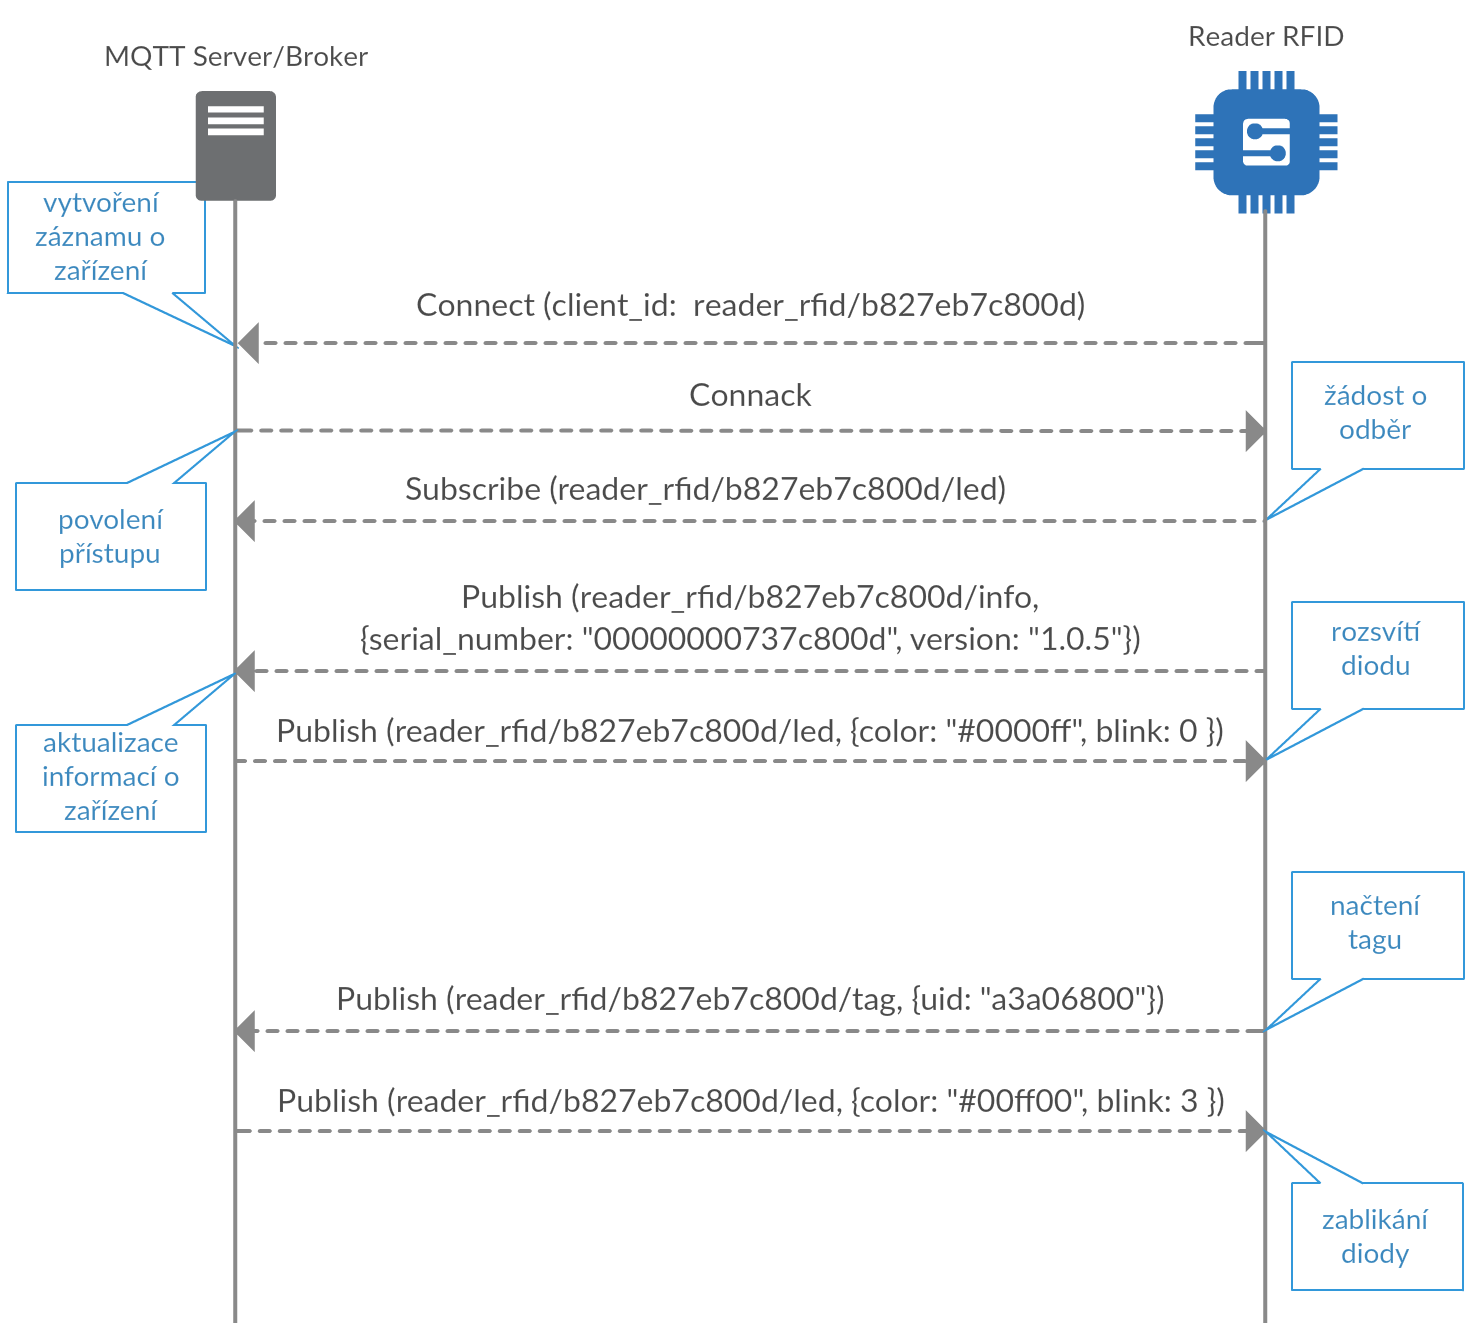
\includegraphics[width=\textwidth]{../diagrams/mqtt_communication.png}	
		\caption{Komunikace mezi čtečkou RFID a MQTT server/broker}
		\label{fig:mqtt_communication}
	\end{figure}





















\chapter{Mobilní aplikace}
	Vývoj mobilní aplikace probíhal nativně v \texttt{Javě} pro \texttt{Android 6.0}.
	Pro zrychlení vývoje jsem použil knihovnu \texttt{Butter Knife}. Její hlavní účel je eliminovat používání metody \texttt{findViewById} pomocí \texttt{property injection @BindView}.
	\texttt{@BindView} do jeho parametru stačí zadat \texttt{ID} požadované komponenty a knihovna \texttt{Butter Knife} automaticky inicializuje \texttt{atribut}. Tímto způsobem jsem dosáhl větší přehlednosti v kódu.
\\\\
Aby aplikace mohla správně fungovat potřebuje tato práva:
\begin{itemize}[noitemsep]
\item [-] INTERNET - umožňuje aplikacím otevřít síťové sokety.
\item [-] ACCESS\_NETWORK\_STATE - umožňuje přístup k informacím o síti.
\item [-] NFC - umožňuje provádět \texttt{I/O} operace přes \texttt{NFC}.
\end{itemize}	
		
\section{Grafické rozhraní}
Do grafického rozhraní jsem zavedl několik vylepšení. Na procházení velkého množství dat byla použita elegantní technika \texttt{infinite scroll}, bez nutnosti čekání se načte další stránka. Princip je jednoduchý, zatímco uživatel skroluje, další obsah je automaticky načítán.
				
Tlačítka jako Uložit, Přihlásit, atd. jsou umístěna v komponentě \texttt{Toolbar}, což je z důvodu dlouhých formulářů, aby nemusel uživatel skrolovat. Takto je tlačítko stále k dispozici.
	
Pro znázornění \texttt{loadingu} byly použity komponenty \texttt{ProgressDialog} a \texttt{ProgressBar}.
\texttt{ProgressBar} se zobrazí při čekání na data od serveru.
\texttt{ProgressDialog} při odesílání dat nejde zrušit kvůli tomu, aby se zabránilo přerušení nebo opětovné operaci. Dialog se zavře, pokud se operace dokončí nebo skončí chybou.

Pro zobrazení dat v přehledech byla použita komponenta \texttt{CardView} pro možnost zobrazit velké množství informací o jednom záznamu. Tímto způsobem jsem se vyhnul prokliku na detaily.

\section{Komunikace}
	Komunikaci s \texttt{REST API} serveru mi zjednodušuje knihovna \texttt{Retrofit}.
	Stačí vytvořit \texttt{Java} rozhraní se všemi možnými dotazy na server a \texttt{Retrofit} si je sám implementuje.
	Požadavky lze volat jako \texttt{Java metody} a přijatá data formátu \texttt{JSON} se konvertují na \texttt{JAVA objekty} pomocí knihovny \texttt{Gson}. 
	Pro editaci \texttt{HTTP hlavičky} jsem použil knihovnu \texttt{OkHttp}. Tato knihovna mi také umožní komunikovat přes \texttt{HTTPS}. 


\section{Lokalizace}
Mobilní aplikace je plně přeložená do dvou jazyků češtiny a angličtiny.
Jazyk se vybírá automaticky podle nastavení v systému a pokud se nenajde požadovaný jazyk, tak se zvolí angličtina. 

Na straně serveru se pracuje s časem bez časových zón.
Aby čas nebyl irelevantní k uživateli, musí se podle časové zóny, kterou má systém \texttt{Android} nastavenou, přepočítat čas.
Toto přináší výhodu, ať je uživatel odkudkoliv, vždy se mu zobrazí správný čas.


%\section{Čtečka NFC}









\chapter{Testování}	
Pro testování mé aplikace pro skladové hospodářství jsem si vybral 6 lidí různého věku a odborného vzdělání. Účastníky testu jsem 
stručně seznámil s funkcemi mé aplikace a zadal jsem jim úkoly, které měli plnit na mobilním zařízení. 
Prvním úkolem bylo přihlásit se do systému aplikace. Administrátorem byl uživatelům dopředu vytvořen účet. Poté měli přidat novou položku skladu. 
Dalším krokem bylo zaevidovat libovolný tag a přidělit mu právě vytvořenou položku. 
Testující použili pro zaevidování tagu různé bezkontaktní karty.  
Posledním úkolem bylo přes čtečku \texttt{RFID} přidat nové položce tři kusy a jeden odebrat.
\\\\
Testování probíhalo na těchto mobilních zařízeních:
\begin{itemize}[noitemsep]
	\item [-] Samsung Galaxy A3 2016 (Android 6.0)
	\item [-] Sony Xperia E5 (Android 6.0)
	\item [-] Huawei P8 Lite (Android 6.0)
\end{itemize}


\section{Výsledky testování}
Účastníci testování, ač byli seznámeni s aplikací jen stručně, si s mobilní aplikací většinou poradili. Nejčastějším problémem se ukázalo, že chtěli přidělit tag k položce, ačkoli to má být opačně. Většina hledala tuto možnost v úpravách položky místo v úpravách tagu. Opačným způsobem to nelze, protože při přidělování tagu k položce bychom nevěděli, jaký tag přidělujeme, což by způsobilo nekonzistentnost dat. Po důkladném vysvětlení se zorientovali a už to pro ně nebyl žádný problém.   
Častý dotaz testujících byl, jak je možné vyhledat konkrétní položku podle názvu. Viz Možnosti rozšíření 
Po objasnění vše velmi dobře zvládli. Nakonec ohodnotili aplikaci jako uživatelsky přívětivou. Testující si vyzkoušeli různé bezkontaktní karty včetně Plzeňské karty. Systém nepřijal karty načtené pomocí mobilní aplikace, jejichž \texttt{UID} bylo delší než 8 znaků, protože to je jiný typ tagu a není podporován čtečkou \texttt{RFID}.   
Vypozoroval jsem, že testujícím chybí některé popisky, nebo že je některé matou. Tyto popisky jsem změnil a např. \uv{Host} byl přejmenován na \uv{Server}.  

Mobilní aplikace fungovala na všech zařízeních bez problémů.


\section{Možnosti rozšíření}
Systém skladového hospodářství potřebuje hodně vylepšení, nejvíce asi aktuální autentizace pro \texttt{API}. Autentizace \texttt{Basic Auth} není dostatečně bezpečná, nahradil bych jí bezpečnější strategií \texttt{OAuth 2.0}, která je ovšem složitější na implementaci.

Dále v tomto systému chybí údaje o tom, kdo vytvořil a upravil záznam v databázi. Tento údaj by pomohl dohledat skladníka, kdy a jak se zbožím manipuloval.

Také bych rozšířil údaje o skladové položce, jelikož nyní obsahuje jen základní údaje: jméno, popisek a množství. Přidal bych např. tyto údaje: cena, expirace a šarže. 
S jiným typem tagu by se otevřela možnost, uložit některé informace do paměti tagu. Tyto informace by mohly být k dispozici i off-line. 

Mobilní aplikaci by prospělo, pokud by v aplikaci bylo vyhledávání v položkách. Z výsledku testování vyplývá, že tato funkce je pro uživatele důležitá a neměla být vynechána.
U tagu je vyhledávání zbytečné, jelikož by šlo vyhledávat jen pomocí \texttt{UID}, což by bylo uživatelsky nepřívětivé. Aktuálně k vyhledání tagu slouží čtečka v mobilní aplikaci. 

Ke zlepšení čtečky \texttt{RFID} by velmi pomohl \texttt{LCD} displej s rozlišením 16x2 znaky. 
\texttt{RGB LED dioda} pro signalizaci stavu čtečky není dostatečná.
Je složité pochopit význam její signalizace. Má omezený počet stavů např. pro odpojení a vypnutí čtečky je stejný stav - zhasnutá \texttt{LED dioda}.
\texttt{LCD} displej by mohl sloužit nejen k zobrazení konkrétního stavu čtečky, ale také k zobrazení informací o tagu a případně o změnách skladové položky.
Takovéto řešení by bylo více uživatelsky přívětivé a cena zařízení by se zvedla jen o 150 korun.

Poslední rozšíření se věnuje posílání informací o zařízení serveru, bylo by vhodné pokud by se posílaly i chybové hlášky. Hlášky by sloužily správci, aby mohl konkrétní zařízení zkontrolovat a případně opravit.

\chapter{Závěr}
Výsledkem mé práce je skladový systém postavený na technologii \texttt{RFID}. Systém se skládá ze tří částí: serveru, čtečky \texttt{RFID} a mobilní aplikace. Server je postavený na \texttt{Node.js}. Komunikaci s dalšími částmi zajišťuje protokol \texttt{MQTT} a \texttt{REST API}. Informace o skladu jsou ukládány do \texttt{NoSQL} databáze \texttt{MongoDB}. Čtečka \texttt{RFID} slouží k přidávání a odebírání skladových položek. Mobilní aplikace pro \texttt{Android} slouží ke správě skladového systému, \texttt{NFC} se využívá k rychlému načtení informací o položce skladu.
\\\\
Pro nasazení skladového systému k praktickému použití by bylo zapotřebí změnit typ \texttt{RFID}. Aktuálně se používá \texttt{HF}. Tento typ \texttt{RFID} je určen např. pro autentizaci.
Pro potřeby skladu je vhodné \texttt{RFID UHF} umožňující ukládat data na tag.
\texttt{UID} tagu by mělo reprezentovat jeden fyzický kus ve skladě a informace o jakou položku se jedná uložit na tag. Další výhodou by byla možnost hromadného načítání.
\\\\
V rámci této práce jsem se seznámil s postupy a technologiemi pro vývoj \texttt{IoT}. Práce ve výsledku splnila zadání, přestože tvorba trvala déle,\\ než se původně předpokládalo.   
Závěrem lze říci, že skladový systém, který vznikl v této práci může dobře sloužit jako prototyp skladového systému pro Průmysl 4.0. 









\chapter*{Přehled zkratek}
\addcontentsline{toc}{chapter}{Přehled zkratek}

	\begin{acronym}[etc]
\acro{API}{Application Programming Interface}
\acro{ASK}{Amplitude Shifting Key}
\acro{BSON}{Bin­ary JSON}
\acro{CRUD}{Create, Read, Update, Delete}
\acro{DOM}{Document Object Model}
\acro{GND}{GrouND}
\acro{GPIO}{General-Purpose Input/Output}
\acro{GUI}{Graphical User Interface}
\acro{HTTP}{Hypertext Transfer Protocol}
\acro{I/O}{Input/Output}
\acro{ID}{Identification}
\acro{IoT}{Internet of Things}
\acro{IP}{Internet Protocol}
\acro{JSON}{JavaScript Object Notation}
\acro{LAN}{Local Area Network}
\acro{LCD}{Liquid-crystal display}
\acro{LED}{Light-Emitting Diode}
\acro{MAC}{Media Access Control}
\acro{NFC}{Near Field Communication}
\acro{NPM}{Node Package Manager}
\acro{NTP}{Network Time Protocol}
\acro{ORM}{Object-relational mapping}
\acro{PyPI}{Python Package Index}
\acro{QoS}{Quality of Service}
\acro{REST}{Representational State Transfer}
\acro{RFID}{Radio Frequency Identification}
\acro{RGB}{Red, Green, Blue}
\acro{RPi}{Raspberry Pi}
\acro{RTC}{Real Time Clock}
\acro{SPI}{Serial Peripheral Interface Bus}
\acro{SSH}{Secure Shell}
\acro{SSL}{Secure Sockets Layer}
\acro{TCP}{Transmission Control Protocol}
\acro{TLS}{Transport Layer Security}
\acro{UID}{Unique Identification}
\acro{URL}{Uniform Resource Locator}
\acro{UWB}{Ultra-Wideband}
\acro{UWP}{Universal Windows Platform}
\acro{XML}{eXtensible Markup Language}
\end{acronym}


\bibliographystyle{csplainnatkiv}
{\raggedright\small
\bibliography{literature}
}








\setcounter{chapter}{0}
\renewcommand{\thechapter}{\Alph{chapter}}%
\chapter{Postup nasazení}

Projekt naleznete na přiloženém DVD nebo je ke stažení na: \\ \url{https://github.com/kohlicekjan/BPINI} 

\section{Server}

\subsection{Instalace}
Pro spuštění serveru je potřeba nainstalovat \texttt{Node.js}. Na oficiálních stránkách je k dispozici podrobný postup: \\
\url{https://nodejs.org/en/download/package-manager/}
\\\\
Pro nainstalování potřebných modulů, spusťte ve složce \texttt{/src/Server/} tento příkaz:
\begin{verbatim}
npm install
\end{verbatim}
\ \\
Nainstalujte také databázi \texttt{MongoDB}, postup naleznete zde: \\
\url{https://docs.mongodb.com/manual/installation/}

\subsection{Konfigurace}
Ve složce projektu \texttt{/src/Server/config} jsou konfigurační soubory. 
V souboru \texttt{default.js} zadejte do \texttt{uri} adresu spuštěné databáze s názvem databáze, kterou chcete vytvořit.
Dále také můžete nastavit adresu a porty serveru. Ukázka konfigurace:
\begin{verbatim}
host: '127.0.0.1',
port: {
    http: 80,
    mqtt: 1883
},
mongodb: {
    uri: 'mongodb://127.0.0.1:27017/warehouse',
    options: {}
}
\end{verbatim}



\subsection{Spuštění}
Server spustíte tímto příkazem:
\begin{verbatim}
node server.js
\end{verbatim}


\section{Čtečka RFID}
	
\subsection{Seznam součástek}
\begin{itemize}
\item 1x Raspberry Pi 2 Model B
\item 1x micro SD karta 
\item 1x RFID-RC522 
\item 1x RGB LED  
\item 3x Resistor 220 Ohm 
\item 11x M-F Kabely samec samice
\item 1x Nepájivé pole
\end{itemize}

\subsection{Zapojení součástek}

Součástky zapojte podle schématu (viz obrázky \ref{fig:reader_rfid_diagram_bb} a \ref{fig:reader_rfid_diagram_schem}).

\begin{figure}[H]
	\centering
	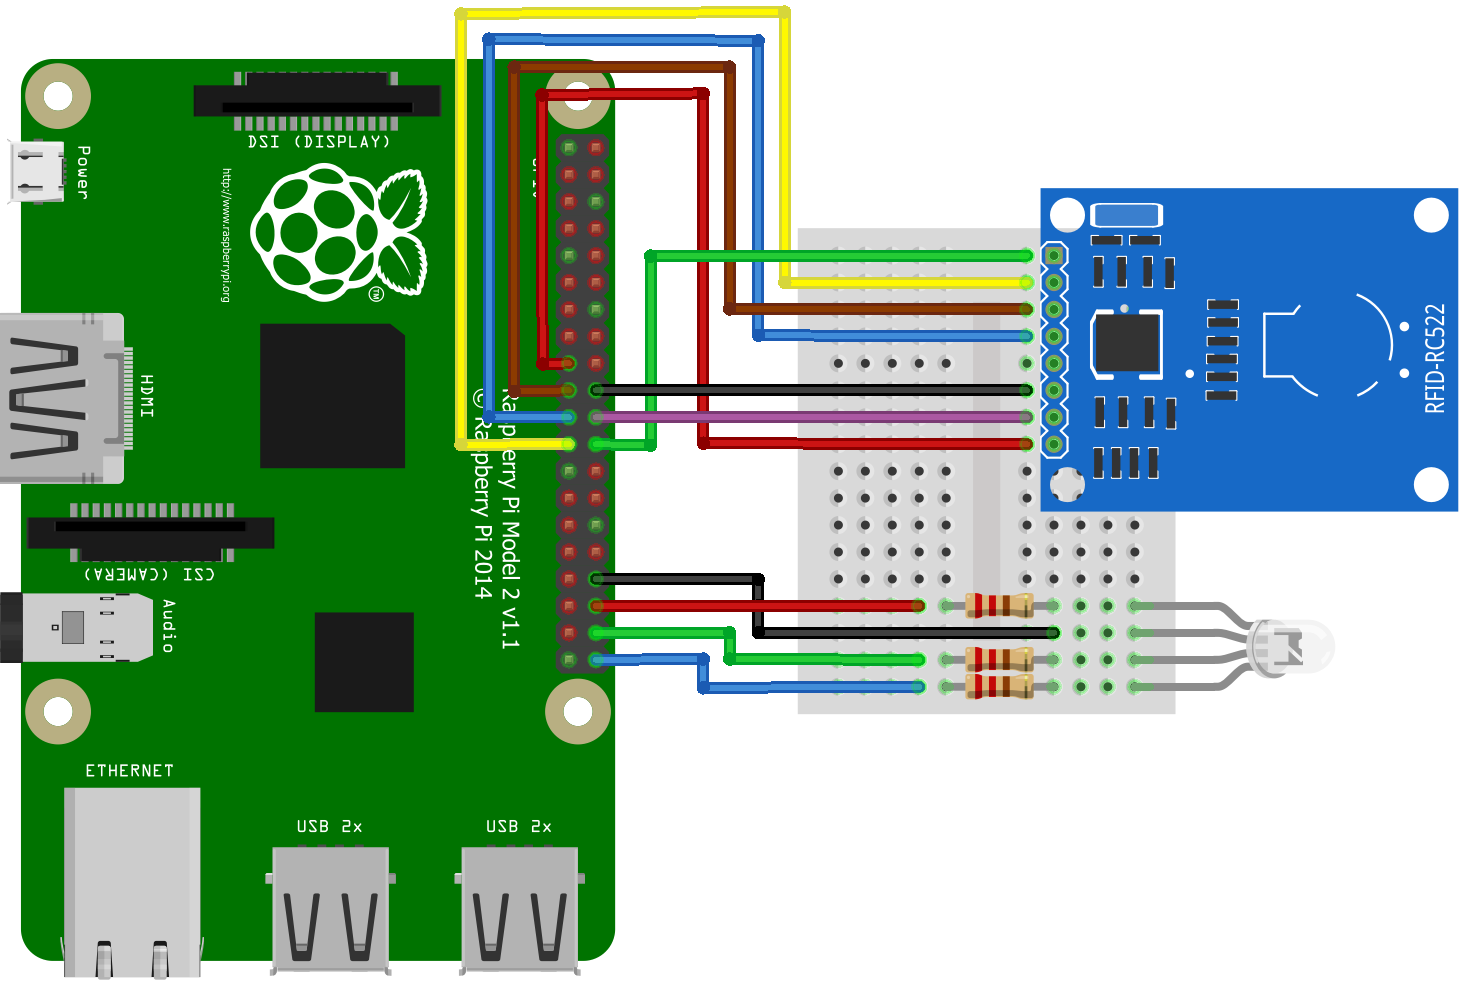
\includegraphics[width=0.9\textwidth]{../diagrams/reader_rfid_diagram_bb.png}	
	\caption{Model čtečky RFID}
	\label{fig:reader_rfid_diagram_bb}
\end{figure}	
	
\begin{figure}[H]
	\centering
	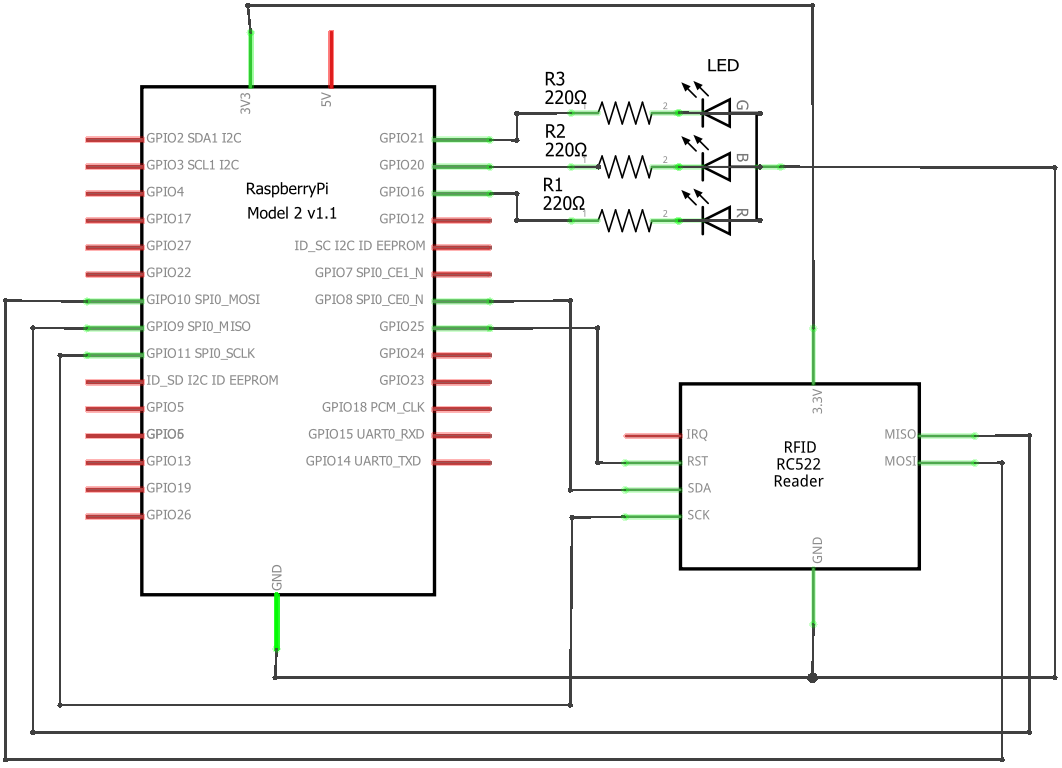
\includegraphics[width=0.9\textwidth]{../diagrams/reader_rfid_diagram_schem.png}	
	\caption{Schéma čtečky RFID}
	\label{fig:reader_rfid_diagram_schem}
\end{figure}

\subsection{Instalace}
Návod na instalaci sytému \texttt{Raspbian Jessie} naleznete na oficiálních stránkách: 
\\ 
\url{https://www.raspberrypi.org/documentation/installation/installing-images/README.md}
\\\\
\texttt{SSH} protokol je z důvodu bezpečnosti ve výchozím stavu zakázán. Návod pro povolení naleznete na stránce: 
\\
\url{https://www.raspberrypi.org/documentation/remote-access/ssh/}
\\\\
V konfiguraci \texttt{Raspberry Pi} povolte tyto položky:
\begin{itemize}[noitemsep]
\item [-] \texttt{Internationalisation Options} -> \texttt{SPI}
\item [-] \texttt{Advanced Options} -> \texttt{GPIO}
\end{itemize}
\ \\
Příkaz pro otevření konfigurace:
\begin{verbatim}
sudo raspi-config
\end{verbatim}
\ \\
\texttt{Python} je součástí \texttt{Raspbianu}, potřebné balíčky se budou instalovat z \texttt{Python Package Index (PyPI)}. K tomu slouží nástroj \texttt{pip}. Tento nástroj je standardně nainstalován v \texttt{Raspbian Jessie} (ale ne \texttt{Jessie Lite}). Můžete jej nainstalovat pomocí příkazu: 
\begin{verbatim}
sudo apt-get install python-pip
\end{verbatim}
\ \\
Následující příkaz nainstaluje všechny potřebné balíčky: 
\begin{verbatim}
sudo pip install -r requirements.txt
\end{verbatim}

\subsection{Spuštění}
Příklad spuštění s nastavením adresy serveru:
\begin{verbatim}
python ./reader_rfid/ -H 10.10.90.26
\end{verbatim}
\ \\
Volitelné parametry:
\begin{itemize}[noitemsep]
	\item \texttt{-h} ... vypíše nápovědu
	\item \texttt{-v} ... vypíše verzi
	\item \texttt{-d} ... zapne logování levelu \texttt{debug}
	\item \texttt{-H} ... adresa serveru
	\item \texttt{-p} ... port pro připojení k serveru
\end{itemize}


\section{Mobilní aplikace}
Aplikace je určena pro \texttt{Android 6.0} a vyšší.	
Soubor \texttt{BPINI-1.4.2.apk} nahrajte do mobilního zařízení a spusťte instalaci.
Při instalaci bude potřeba dočasně povolit \texttt{instalaci z neznámých zdrojů}.
Po dokončení najdete aplikaci v menu mezi ostatními aplikacemi.


\chapter{Uživatelský manuál}

	\section{Čtečka RFID}
Čtečka svůj stav signalizuje pomocí \texttt{LED diody} její stavy (viz tabulka \ref{table:led_states}).

\begin{table}[H]
\centering
\begin{tabular}{ c | p{6cm} }
\textbf{LED dioda} & \textbf{Popis} \\ \hline\hline
vypnuta & není navázáno připojení \\ \hline  
svítí zelená & režim přidávání položek \\ \hline
svítí červeně & režim odebírání položek \\ \hline
bliká zeleně & akce proběhla úspěšně \\ \hline
bliká červeně & nastala nečekaná chyba  \\ \hline
bliká modře & tag nemá nastavenou žádnou funkci  \\ \hline
\end{tabular}
\caption{Stavy LED diody}
\label{table:led_states}
\end{table}
\ \\
Tag načtený čtečkou se automaticky zaeviduje. Funkčnost tagu potom můžeme nastavit v mobilní aplikaci.
Je-li čtečka v režimu přidávání položek a načte-li tag reprezentující položku, přičte se k položce +1 množství.
K přepínání režimů slouží speciální tag typu \uv{režim}.

\newpage

\section{Mobilní aplikace}
	
\subsection{Přihlášení}	
Při prvním spuštění aplikace se zobrazí přihlašovací formulář (viz obrázek \ref{fig:Screenshot_20170610-134211}).
Zadejte adresu serveru, pak následuje uživatelské jméno a heslo (viz obrázek \ref{fig:Screenshot_20170612-002041}). 
\\\\
Výchozí přihlašovací údaje administrátora systému jsou:
\begin{itemize}[noitemsep]
\item [-] uživatelské jméno: admin
\item [-] heslo: heslo
\end{itemize}
\begin{figure}[H]
	\centering
  \begin{subfigure}[b]{0.3\textwidth}
    \centering
	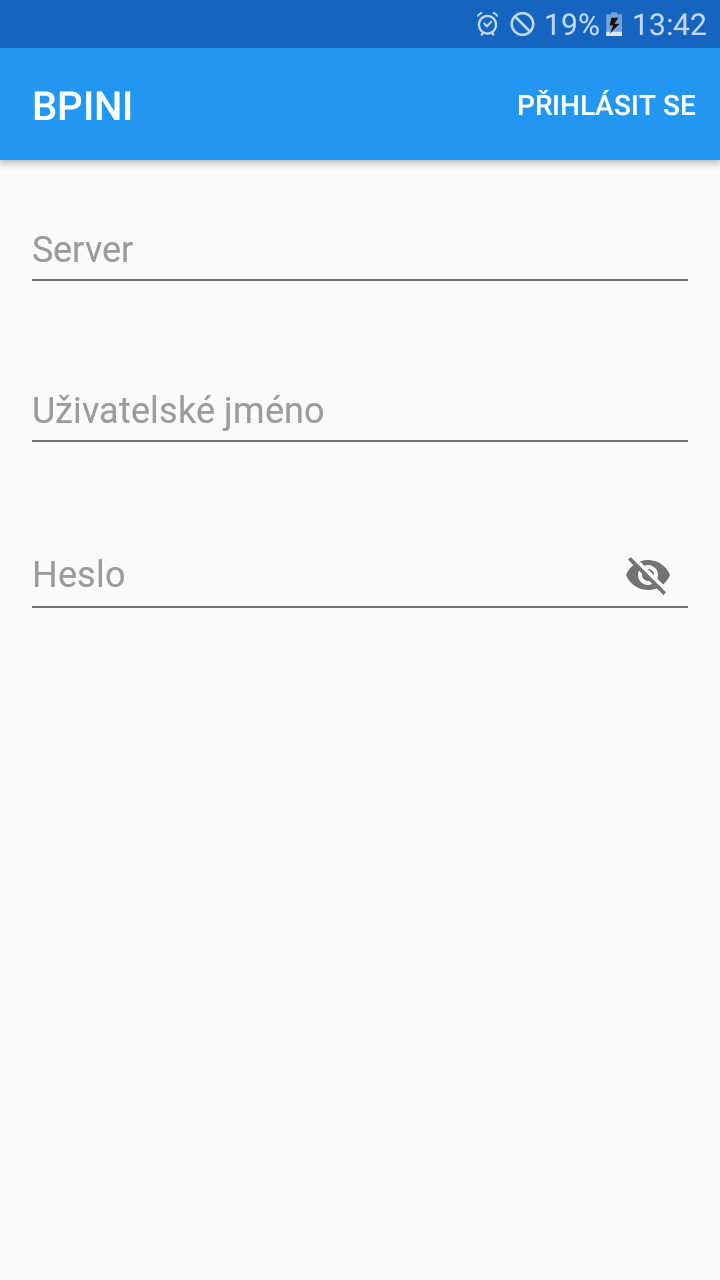
\includegraphics[width=\textwidth]{../images/client_android/Screenshot_20170610-134211.png}	
	\caption{Prázdný}
	\label{fig:Screenshot_20170610-134211}
  \end{subfigure}
  %
  \begin{subfigure}[b]{0.3\textwidth}
    \centering
	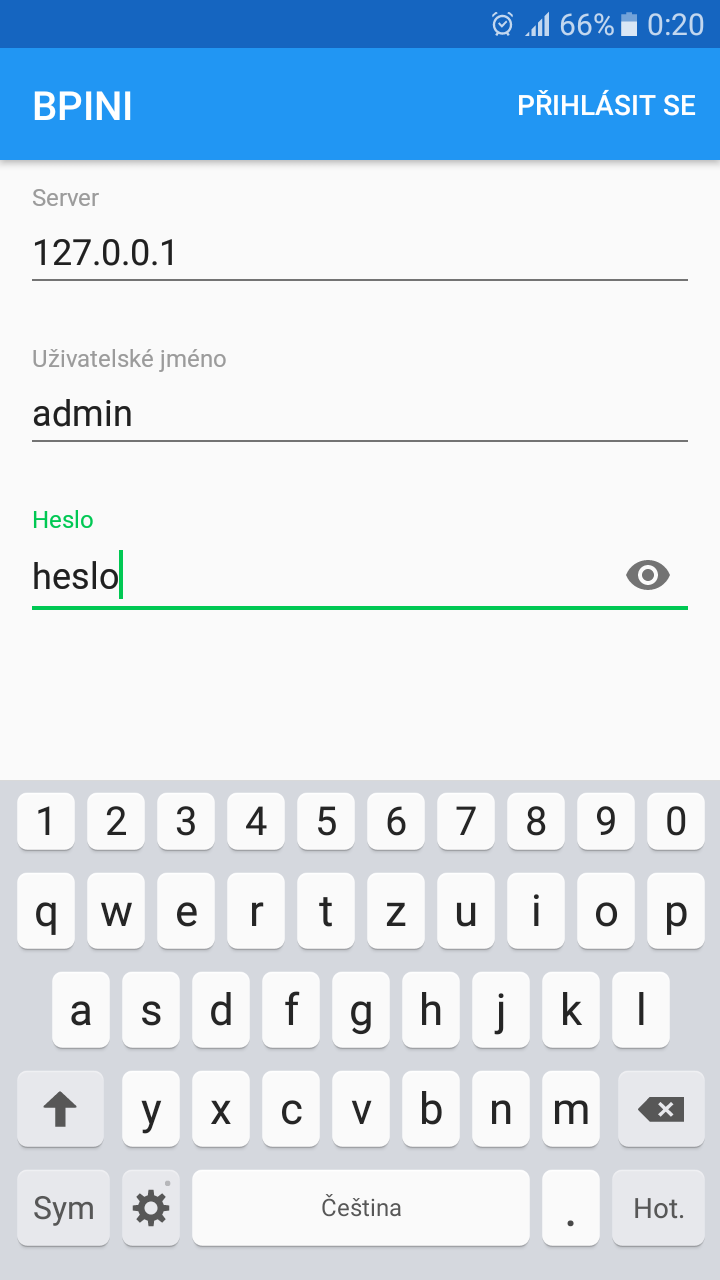
\includegraphics[width=\textwidth]{../images/client_android/Screenshot_20170612-002041.png}	
	\caption{Vyplněný}
	\label{fig:Screenshot_20170612-002041}
  \end{subfigure}
  \caption{Přihlašovací formulář}
\end{figure}


\subsection{Menu}
Menu se zobrazí stisknutím hamburger menu nebo vysunutím zpoza okraje (viz obrázek \ref{fig:Screenshot_20170607-164924}).
První položka menu otevírá detail přihlášeného uživatele.
Na  řádce jsou výše zmíněné \uv{Položky}, pak následují \uv{Tagy}.
Další položkou v menu je \uv{Čtečka}, ta je dostupná jen pro mobilní zařízení s \texttt{NFC}, ostatním se nezobrazí.
Poté následují \uv{Zařízení} a \uv{Uživatelé}, které jsou přístupné jen pro administrátora.
Poslední je \uv{O aplikaci}, zobrazí verzi, popis a autora aplikace.
\begin{figure}[h]
	\centering
	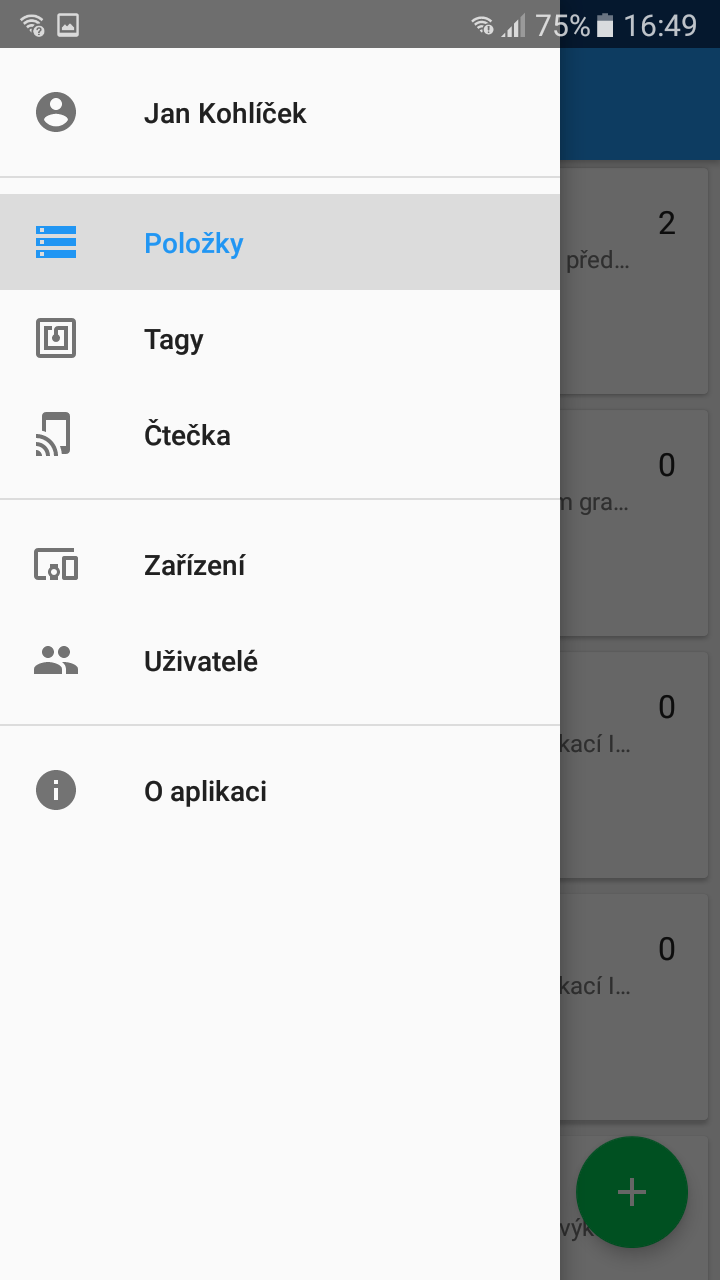
\includegraphics[width=0.3\textwidth]{../images/client_android/Screenshot_20170607-164924.png}	
	\caption{Menu aplikace}
	\label{fig:Screenshot_20170607-164924}
\end{figure}



\subsection{Položky}	
Po spuštění aplikace se zobrazí seznam položek skladu (viz obrázek \ref{fig:Screenshot_20170607-164919}).
Položky můžete přidat pomocí zeleného plus v pravém dolním rohu a kliknutím na danou položku editovat.
Položku lze smazat jen tehdy, když se její počet rovná nule.
\begin{figure}[H]
	\centering
  \begin{subfigure}[b]{0.3\textwidth}
    \centering
	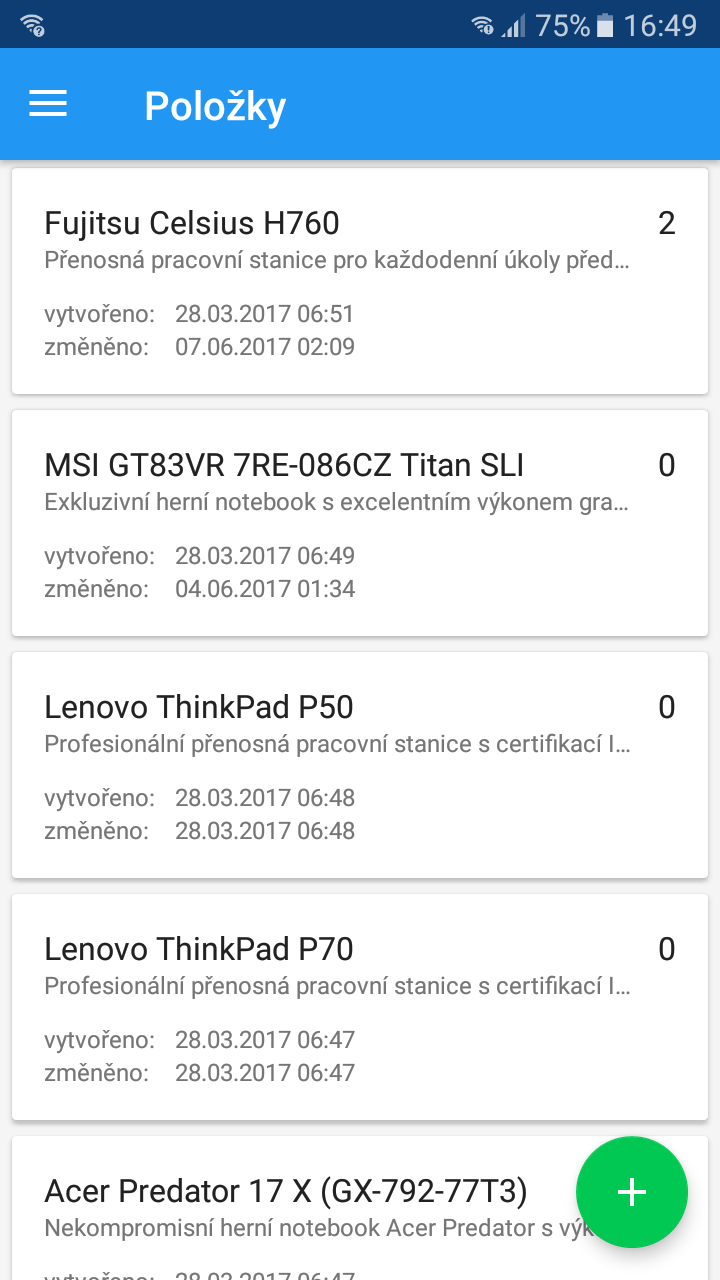
\includegraphics[width=\textwidth]{../images/client_android/Screenshot_20170607-164919.png}	
	\caption{Seznam položek}
	\label{fig:Screenshot_20170607-164919}
  \end{subfigure}
  %
  \begin{subfigure}[b]{0.3\textwidth}
    \centering
	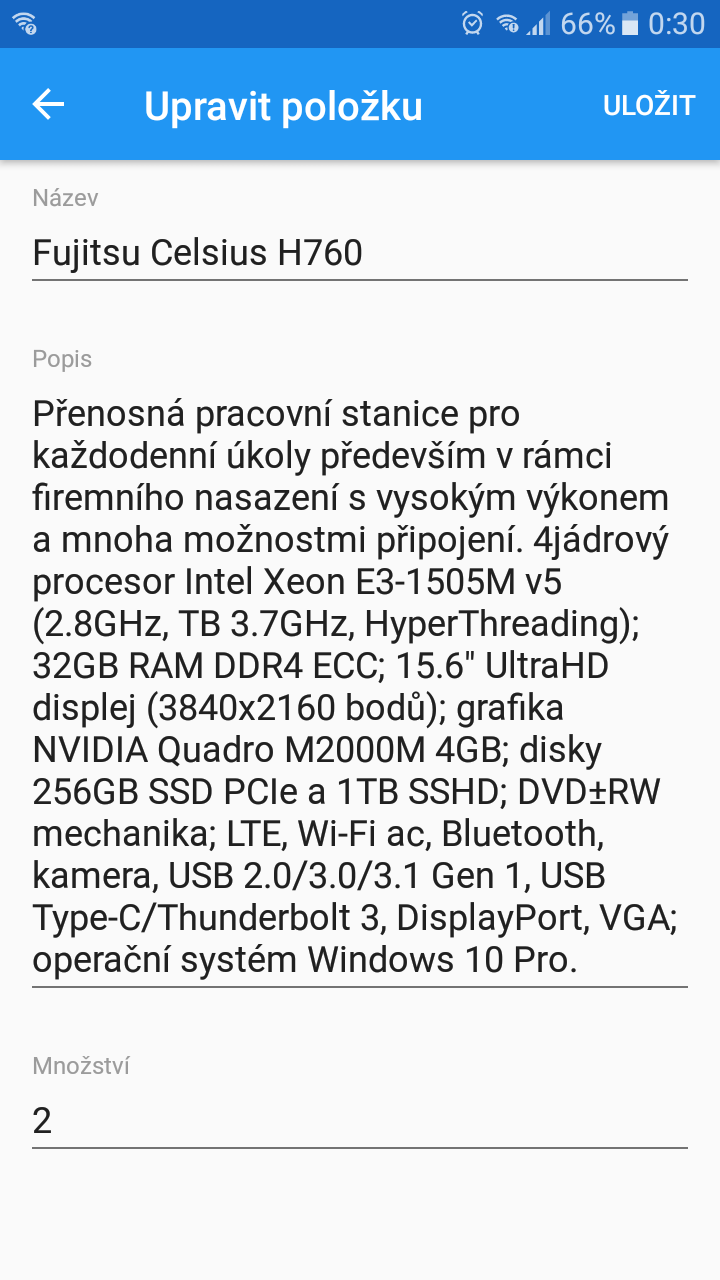
\includegraphics[width=\textwidth]{../images/client_android/Screenshot_20170612-003030.png}	
	\caption{Úprava položky}
	\label{fig:Screenshot_20170612-003030}
  \end{subfigure}
  \caption{Položky}
\end{figure}



\subsection{Tagy}
Tagy nelze přidávat ručně, jen pomocí čtečky. Kliknutím na tag se zobrazí editace (viz obrázek \ref{fig:Screenshot_20170607-165805}), která nabízí změnu typu. Tag může být tří typů:
\begin{description}
\item [neznámý] - tag nemá nastavenou žádnou funkci
\item [režim] - tag umožňuje čtečce RFID přepínat režimy přidat/odebrat položku
\item [položka] - tag reprezentuje položku ve skladu 
\end{description}
\begin{figure}[H]
	\centering
  \begin{subfigure}[b]{0.3\textwidth}
    \centering
	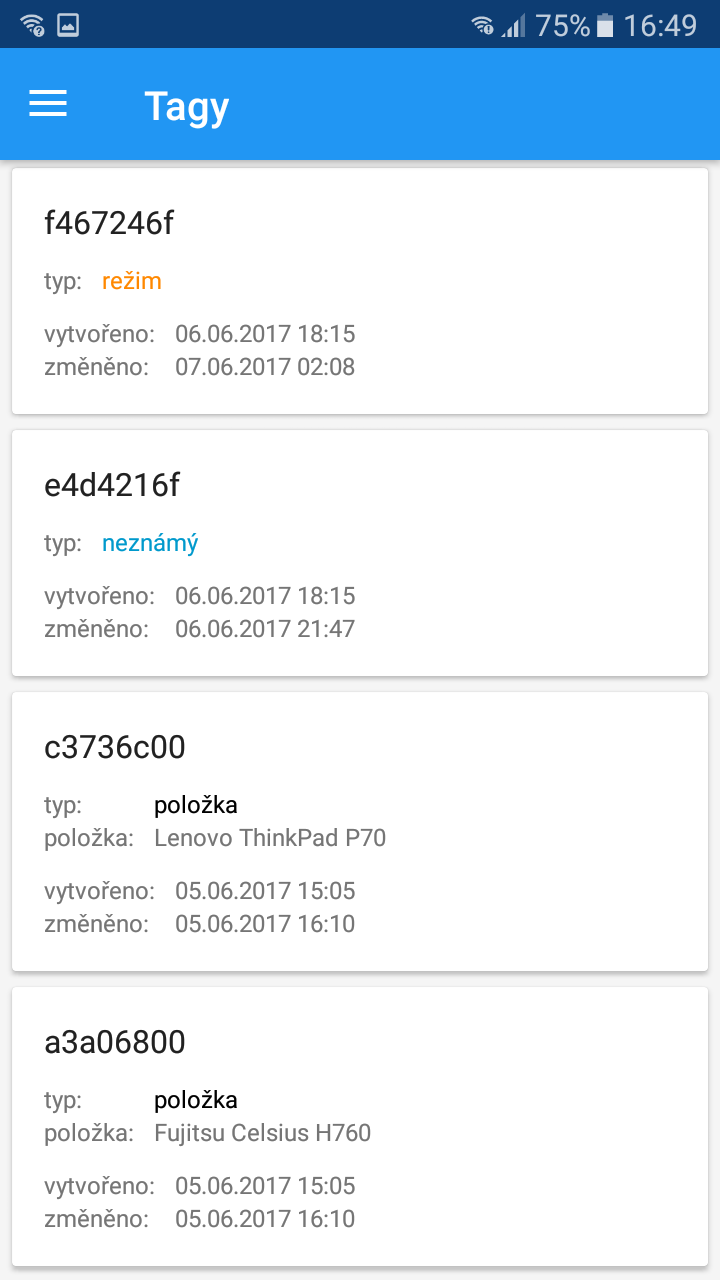
\includegraphics[width=\textwidth]{../images/client_android/Screenshot_20170607-164958.png}	
	\caption{Seznam tagů}
	\label{fig:Screenshot_20170607-164958}
  \end{subfigure}
  %
  \begin{subfigure}[b]{0.3\textwidth}
    \centering
	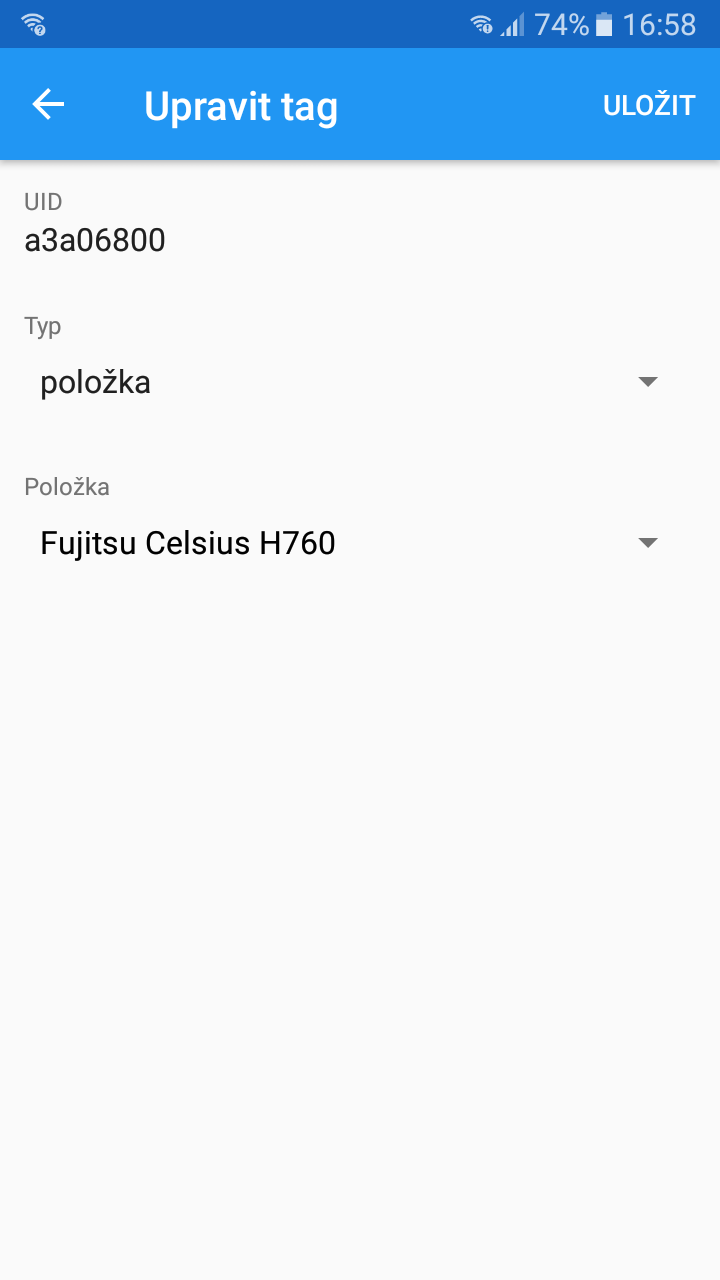
\includegraphics[width=\textwidth]{../images/client_android/Screenshot_20170607-165805.png}	
	\caption{Úprava tagu}
	\label{fig:Screenshot_20170607-165805}
  \end{subfigure}
  \caption{Tagy}
\end{figure}


\subsection{Čtečka}
Čtečka čekající na přiložení tagu (viz obrázek \ref{fig:Screenshot_20170607-165058}).
Po přiložení tagu se načtou detailní informace (viz obrázek \ref{fig:Screenshot_20170607-165117}), ale pokud není v systému zaevidován, pak je vytvořen tag typu \uv{neznámý}.
\begin{figure}[H]
	\centering
  \begin{subfigure}[b]{0.3\textwidth}
    \centering
	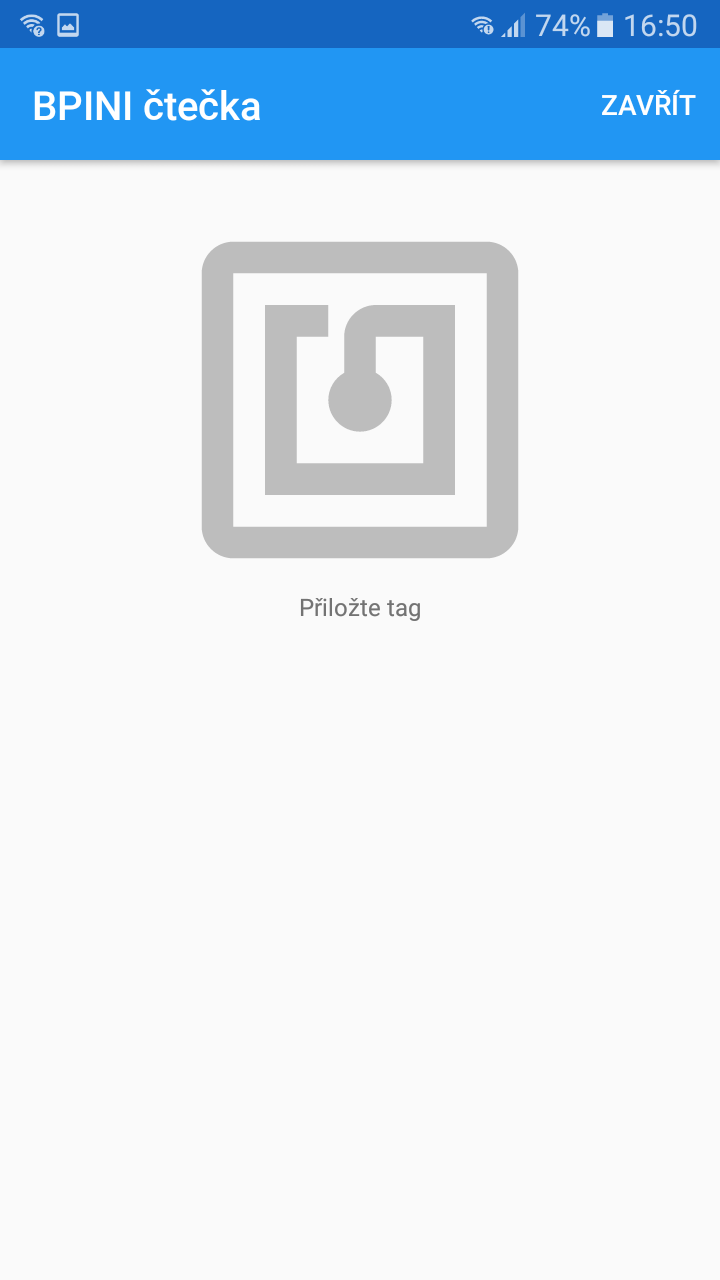
\includegraphics[width=\textwidth]{../images/client_android/Screenshot_20170607-165058.png}	
	\caption{Připravená čtečka}
	\label{fig:Screenshot_20170607-165058}
  \end{subfigure}
  %
  \begin{subfigure}[b]{0.3\textwidth}
    \centering
	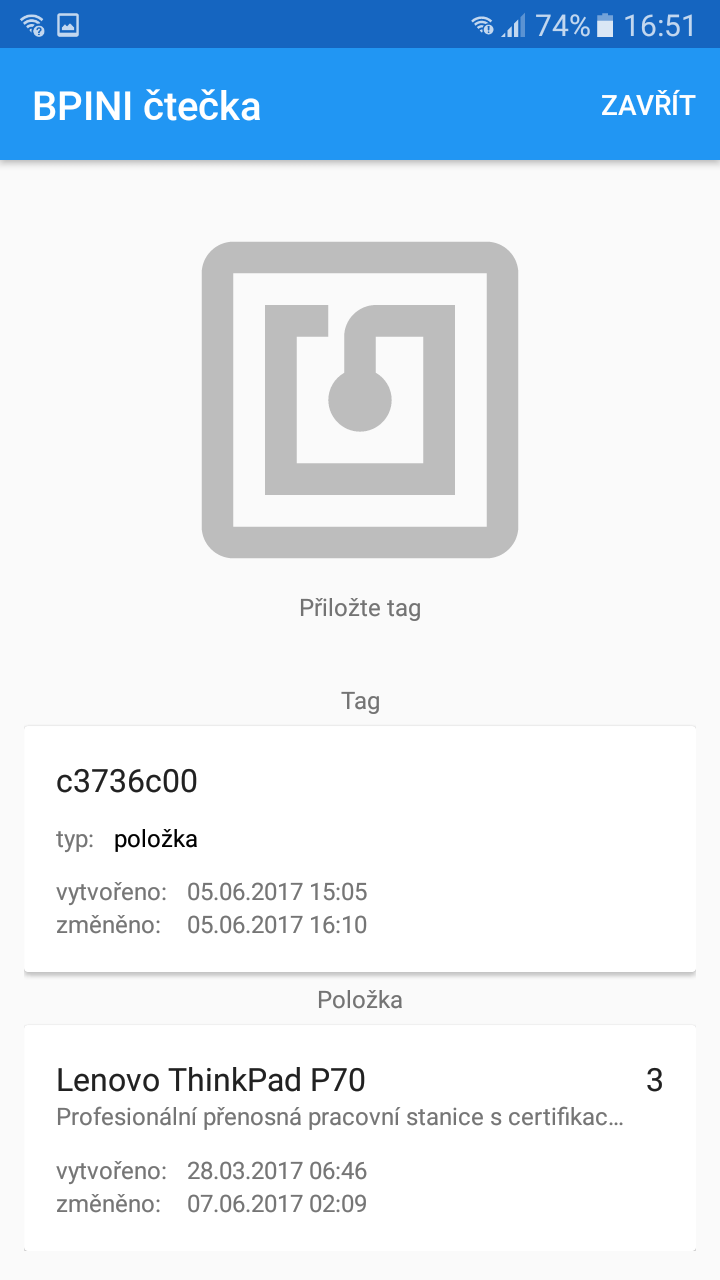
\includegraphics[width=\textwidth]{../images/client_android/Screenshot_20170607-165117.png}	
	\caption{Načtený tag}
	\label{fig:Screenshot_20170607-165117}
  \end{subfigure}
  \caption{Čtečka}
\end{figure}


\subsection{Administrace}
Seznam zařízení se ukazuje jen administrátorům (viz obrázek \ref{fig:Screenshot_20170607-165221}). Zařízení se evidují automaticky při jakémkoli pokusu o připojení k serveru. Aby se zařízení připojilo, je nutné, aby konkrétnímu zařízení byl povolen přístup. Ten se mění pomocí přepínače.
\begin{figure}[H]
	\centering
	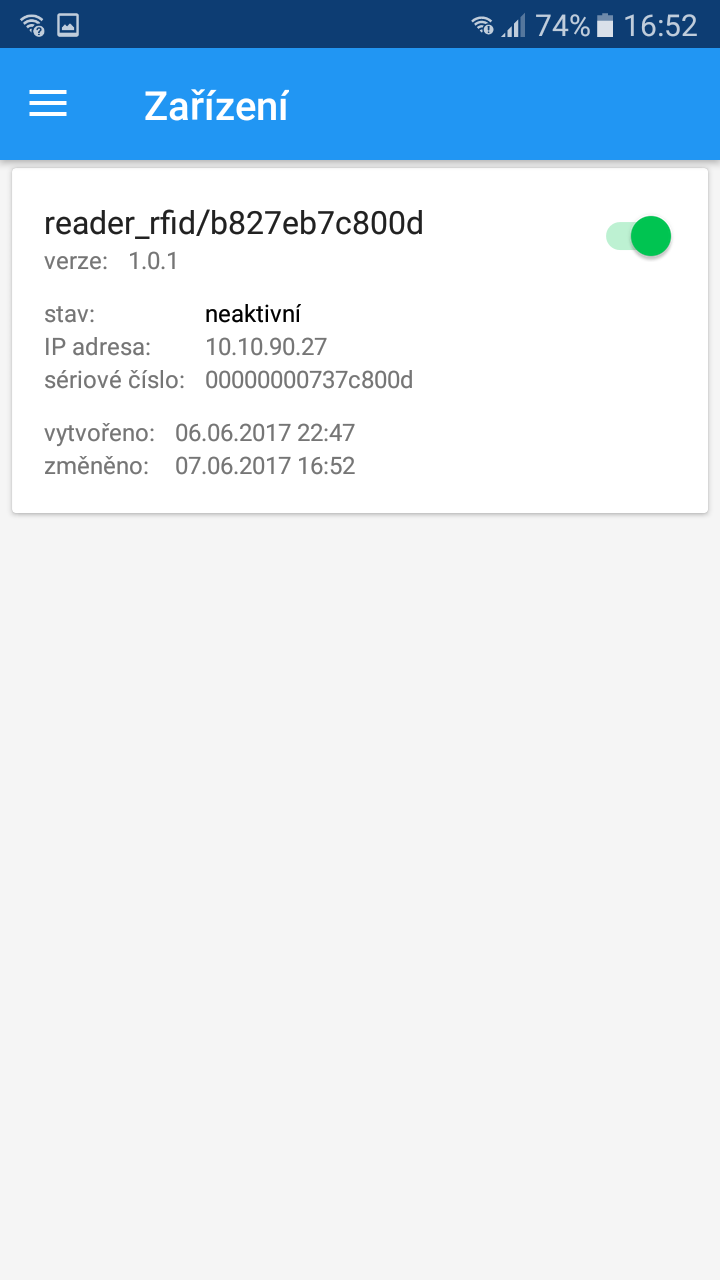
\includegraphics[width=0.3\textwidth]{../images/client_android/Screenshot_20170607-165221.png}	
	\caption{Zařízení}
	\label{fig:Screenshot_20170607-165221}
\end{figure}
\ \\
Jen administrátor má přístup ke správě uživatelů (viz obrázek \ref{fig:Screenshot_20170607-165248}).
Dostat se na vytvoření nového uživatele je možné přes zelené plus v pravém dolním rohu a kliknutím na uživatele editovat.
Uživatele s rolí \uv{administrátor} může vytvářet a editovat jen výchozí administrátor.
\begin{figure}[H]
	\centering
  \begin{subfigure}[b]{0.3\textwidth}
	\centering
	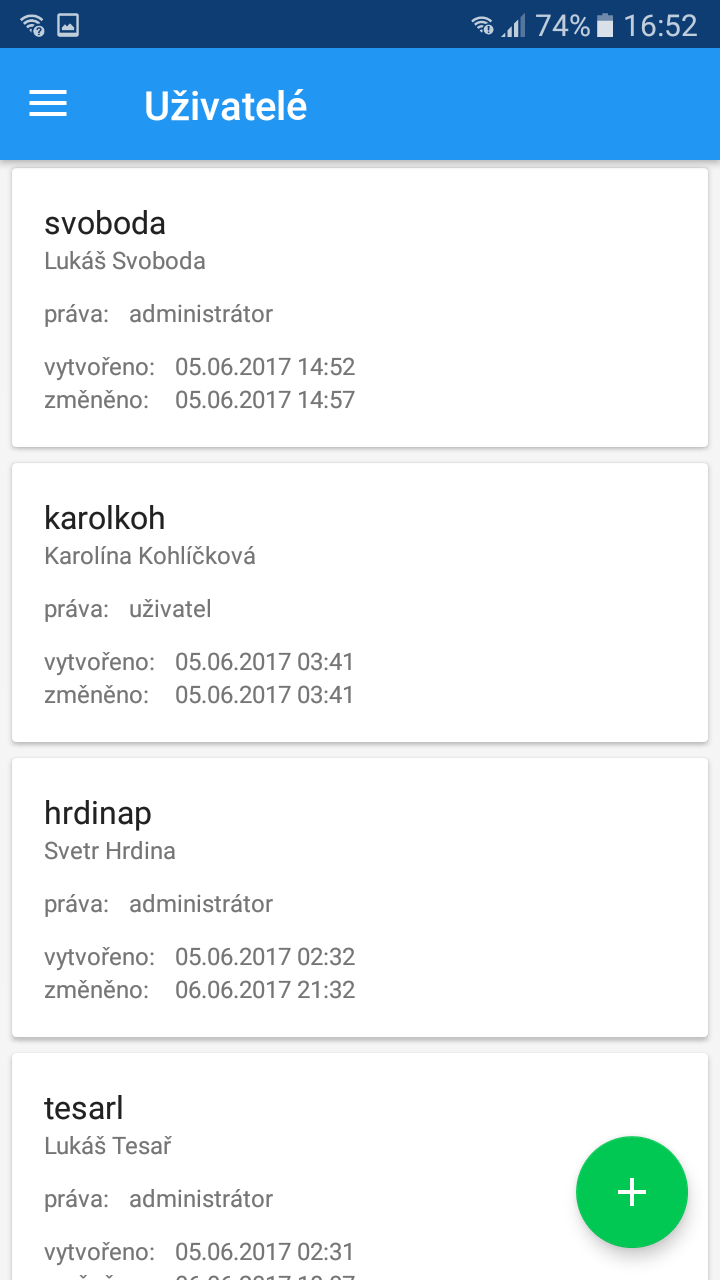
\includegraphics[width=\textwidth]{../images/client_android/Screenshot_20170607-165248.png}	
	\caption{Seznam uživatelů}
	\label{fig:Screenshot_20170607-165248}
  \end{subfigure}
  %
  \begin{subfigure}[b]{0.3\textwidth}
    \centering
	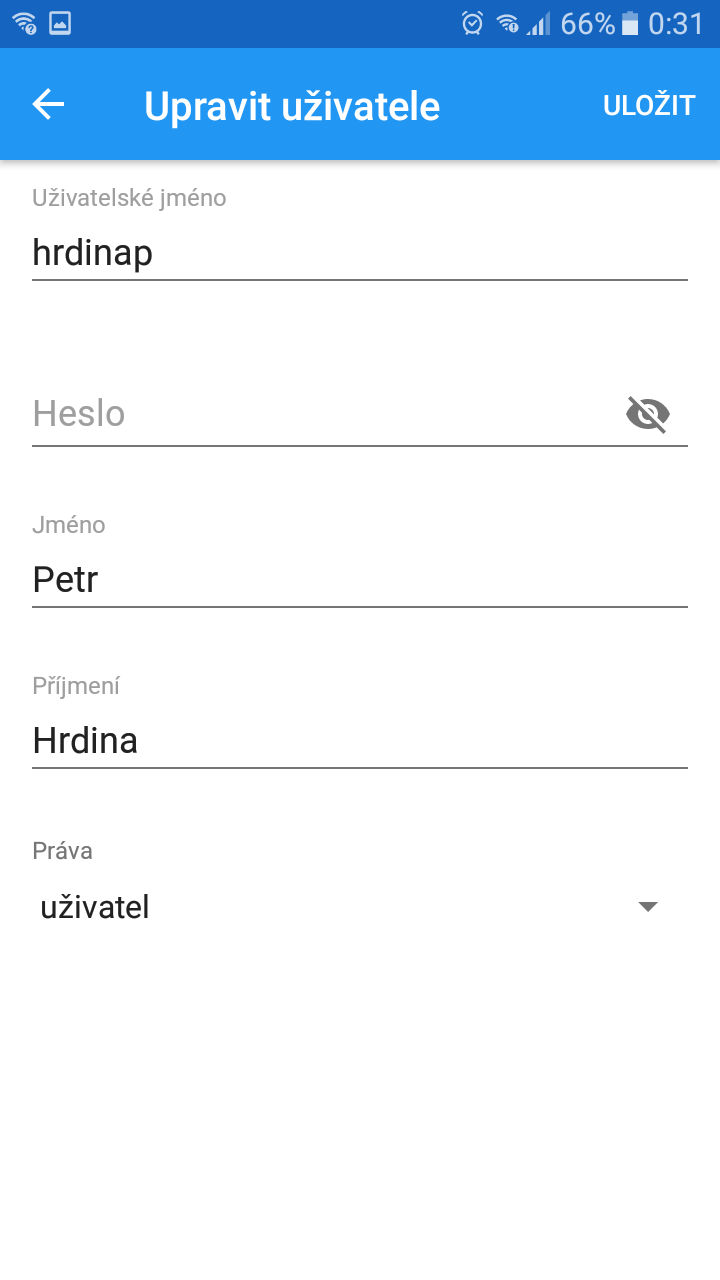
\includegraphics[width=\textwidth]{../images/client_android/Screenshot_20170612-003127.png}	
	\caption{Úprava uživatele}
	\label{fig:Screenshot_20170612-003127}
  \end{subfigure}
  \caption{Uživatelé}
\end{figure}



\chapter{Obsah přiloženého CD}
Obsah \texttt{CD} je k dispozici na \url{https://github.com/kohlicekjan/BPINI}.
\\\\
Popis adresářové struktury:
\begin{itemize}[noitemsep]
\item [-] \texttt{build}
	\begin{itemize}[noitemsep]
		\item [+] \texttt{ClientAndroid} - instalační balíčky mobilní aplikace
	\end{itemize}
\item [-] \texttt{docs}
	\begin{itemize}[noitemsep]
		\item [+] \texttt{bpini} - text bakalářské práce
		\item [+] \texttt{diagrams} - diagramy
		\item [+] \texttt{images} - obrázky 
	\end{itemize}
\item [-] \texttt{src}
	\begin{itemize}[noitemsep]
		\item [+] \texttt{ClientAndroid} - zdrojové kódy mobilní aplikace pro \texttt{Android}
		\item [+] \texttt{ReaderRFID} - zdrojové kódy čtečky \texttt{RFID} pro \texttt{Raspberry Pi}
		\item [+] \texttt{Server} - zdrojové kódy serveru
	\end{itemize}
\end{itemize}


\end{document}
